%! Author = user
%! Date = 01.11.23

% Preamble
\documentclass[11pt]{report}

\title{Compiler Development for LR(1) Grammars: \(DK_{1}\) Test, Parsing, and Code Generation with Application to the \(C0\) Language\\ \vspace{10pt}{\Large Kutaisi International University}}
\author{Irakli Khotchava\\Toma Pirtskhelani \vspace{30pt}\\ Supervisor:\\ Wolfgang J. Paul}
\date{}

% Packages
\usepackage{amsmath, amsfonts, amsthm}
\usepackage{graphicx}
\usepackage{verbatim}
\usepackage{fancyvrb}
\usepackage{tikz}
\usepackage{listings}
\usepackage{array}
\usepackage[colorlinks = true,
    linkcolor = black,
    urlcolor  = blue,
    citecolor = blue]{hyperref}
\usepackage{fullpage}
\usepackage{calc}
\usepackage{amssymb}
\usepackage{stmaryrd}
\usetikzlibrary{positioning,shadows,arrows,trees,shapes,fit}
\usetikzlibrary{graphs} % LaTeX and plain TeX
\usetikzlibrary[graphs] % ConTeXt
\usetikzlibrary{decorations.pathreplacing}
\VerbatimFootnotes

\lstnewenvironment{codeblock}[1][]
{\lstset{
    language=Java, % Change this to the programming language you're using
    basicstyle=\small\ttfamily,
    numbers=left,
    numberstyle=\tiny,
    numbersep=5pt,
    keywordstyle=\color{blue!50!black},
    commentstyle=\color{black!70!},
    stringstyle=\color{blue!50!black},
    showstringspaces=false,
    breaklines=true,
    frame=single,
    captionpos=b,
    caption=#1,
}
}
{}

\tikzset {
    style A/.style={
        top color=white,
        bottom color=white!25,
        draw=black,
        thick,
        rectangle, % Set the shape as a rectangle
        minimum size=6mm,
        align=center,
    },
    style B/.style={
        top color=white,
        bottom color=white!25,
        draw=black,
        thick,
        rectangle, % Set the shape as a rectangle
        rounded corners=.2cm,
        minimum size=10mm,
        align=center,
    },
    style C/.style={
        top color=green!65!black,
        bottom color=green!65!black,
        draw=green!65!black,
        thick,
        color=white,
        rectangle, % Set the shape as a rectangle
        minimum size=8mm,
        align=center,
    },
    style D/.style={
        top color=red!80!black,
        bottom color=red!80!black,
        draw=red!80!black,
        thick,
        color=white,
        rounded corners=.2cm,
        rectangle, % Set the shape as a rectangle
        minimum size=10mm,
        align=center,
    },
}

\newtheorem*{definition}{Definition}

\newcommand{\tok}[1]{\langle #1 \rangle}
\newcommand{\sep}{\ |\ }

% Document
\begin{document}
    \maketitle

    \tableofcontents
    \chapter{Introduction}\label{ch:Introduction}

% Overview
\section*{Overview}
This thesis introduces an entire compiler development for languages derived from LR(1) grammars. It involves:

\begin{itemize}
    \item Lexical analysis of both the source code and the input context-free grammar(CFG).
    \item Testing whether the input CFG is indeed LR(1).
    \item The source code pre-processing.
    \item Syntactic analysis, where the parser examines the refined token sequence to decode its hierarchical structure. The outcome is the parse tree, representing the complete hierarchical structure of the source code as per the input programming language's grammar.
    \item The thesis details the implementation of a data structure to store CFGs and the construction of a \({DK_{1}}\) automaton, as advised by Michael Sipser \cite{sipser}, to test the LR(1) status of the input grammar.
    \item The latter part of the thesis addresses the compiler backend, focusing on data structures for symbol tables and assembly generation from the provided derivation tree.
    \item At the end of the thesis you will see the compiled C0 codes.
\end{itemize}

% Focus
\section*{Focus}
Our study concentrates on the \(C0\) language, which merges \(C\)'s syntax with \(Free Pascal\)'s semantics. This language is defined using context-free grammar (CFG), as illustrated in \hyperref[fig:grammar_c0]{Figure 1.1}. We will test the language's ambiguity and then classify it according to LR(1) grammar. This will lead to the development of a detailed compiler, which we will implement using the \(Java\) programming language.

% Methodology and Implementation
\section*{Methodology and Implementation}
Our methodology and implementation are based on these books:
\begin{itemize}
    \item "System Architecture: An Ordinary Engineering Discipline" by Sabine Schmaltz, Petro Lutsyk, Wolfgang J. Paul. \cite{sysbook}
    \item "Introduction to the Theory of Computation"
    by Michael Sipser. \cite{sipser}
\end{itemize}
\setlength{\parindent}{0pt}

Leveraging this theoretical groundwork, we've designed an LR(1) context-free grammar tester and parser to process not just \(C0\) language, but also all other languages specified by CFGs, including \(C\), \(Java\), and the like.\\

The entire implementation in Java is accessible on \href{https://github.com/fyfsb/dcfg.git}{GitHub}.

\begin{itemize}
    \item The \hyperref[ch:Lexical and Syntactic Analysis]{Chapter 2} and all the corresponding code development is done by Toma Pirtskhelani.
    \item The \hyperref[ch:backend]{Chapter 3} and all the corresponding code development is done by Irakli Khotchava.
\end{itemize}

% C0 CFG
\begin{figure}[h!]
    \center
    \includegraphics[width=13cm]{C0.png}
    \caption{C0 Context-Free Grammar}
    \label{fig:grammar_c0}
\end{figure}
    \chapter{Lexer and Parser}\label{ch:Lexer and Parser}

\newpage


% Structure Implementation for Context-Free Grammars
\section{Structure Implementation for Context-Free Grammars}\label{sec:Structure Implementation for Context-Free Grammars}

Before diving into language ambiguity testing and source code parsing, we need to properly read and accurately store the input grammar. A precise specification and understanding of the source grammar are fundamental for our parser’s architecture.\\

% Context-Free Grammar Definition
\begin{definition}[1.0]
    A context-free grammar is a 4-tuple \((N, T, P, S)\), where
    \begin{enumerate}
        \item \(N\) is a finite set called the nonterminal symbols,
        \item \(T\) is a finite set, disjoint from N, called the terminal symbols,
        \item \(P\) is a finite set of production rules, with each rule being a nonterminal deriving a string of terminal and/or nonterminal symbols,
        \item \(S \in N\) is the start nonterminal symbol.
    \end{enumerate}
\end{definition}
\setlength{\parindent}{0pt}

Given this definition of a context-free grammar, our implementation will replicate its structure to properly follow the mathematical theory used in this thesis.\\

For proper replication, we create these three classes:
\begin{enumerate}
    \item Class \(\boldsymbol{Symbol}\): \textit{Both terminal and nonterminal symbols are atomic elements of CFGs. Thus, we might want to create a class that will encapsulate these elements properly.}
    \item Class \(\boldsymbol{Production}\): \textit{In CFGs, production rules dictate how a nonterminal symbol can be replaced by a sequence of terminal and/or nonterminal symbols. Therefore, we need a class that will encapsulate the concept of a production rule.}
    \item Class \(\boldsymbol{Grammar}\): \textit{This class represents the entire CFG. \(\boldsymbol{Grammar}\) should replicate the mathematical definition of CFGs.}
\end{enumerate}

For a convenient implementation design, we group these three classes under a package named \(\boldsymbol{grammar}\).\\

Now let’s explore each of these classes in detail.

% Symbol Class
\subsection*{\(\boldsymbol{Symbol}\) Class}

The \(\boldsymbol{Symbol}\) class encapsulates the concept of terminal and nonterminal symbols. In CFGs, terminal and nonterminal symbols are strings. The input grammar explicitly determines which of the symbols are terminal and which are nonterminal.\\
Thus, to properly encapsulate the concept of a symbol of a CFG, we need an attribute for the string content and another attribute for the type of the symbol (terminal / nonterminal).\\

\textbf{Attributes:}
\begin{itemize}
    \item \(\boldsymbol{content}\): \textit{A string representing the actual content of the symbol.}
    \item \(\boldsymbol{type}\): \textit{An enum indicating whether the symbol is a terminal or nonterminal.}
\end{itemize}

We also present some basic methods to further simplify and shorten the overall implementation of the parser.\\

\textbf{Methods:}
\begin{itemize}
    \item \(\boldsymbol{constructor}\): \textit{Initializes a \(\boldsymbol{Symbol}\) object with the specified content and type.}
    \item \(\boldsymbol{isTerminal}\): \textit{Returns true if the symbol is terminal, returns false otherwise.}
    \item \(\boldsymbol{length}\): \textit{Returns the length of the content string.}
    \item \(\boldsymbol{equals}\): \textit{Determines whether two \(\boldsymbol{Symbol}\) objects are equal in both content and type.}
    \item \(\boldsymbol{hashCode}\): \textit{Returns a hash code of the symbol.}
\end{itemize}

\begin{codeblock}[Symbol Class]
    class Symbol {
        enum SymbolType {
            Terminal, Nonterminal
        }
        String content;
        SymbolType type;

        Symbol(String content, SymbolType type) {}
        boolean isTerminal() {}
        int length() {}
        boolean equals(Object obj) {}
        int hashCode() {}
    }
\end{codeblock}

\vspace{10pt}

% Production Class
\subsection*{\(\boldsymbol{Production}\) Class}

The \(\boldsymbol{Production}\) class encapsulates the concept of a production rule of a CFG. A representation of a production rule has the form:

\begin{verbatim}
left (nonterminal) → right (sequence of terminals and/or nonterminals)
\end{verbatim}

meaning – the right-hand side sequence can be derived from the left-hand side nonterminal. Therefore, to properly encapsulate a production rule we need two attributes: a left-hand side nonterminal and a right-hand side sequence of symbols.\\


\textbf{Attributes:}
\begin{itemize}
    \item \(\boldsymbol{left}\): \textit{A nonterminal \(\boldsymbol{Symbol}\) representing the left-hand side of the production.}
    \item \(\boldsymbol{right}\): \textit{An Array List of \(\boldsymbol{Symbol}\) objects representing the sequence of terminals and/or nonterminals on the right side of the production.}
\end{itemize}

\textbf{Methods:}
\begin{itemize}
    \item \(\boldsymbol{constructor}\): \textit{Initializes a \(\boldsymbol{Production}\) object with the specified left and right attributes.}
    \item \(\boldsymbol{equals}\): \textit{Determines if two \(\boldsymbol{Production}\) objects are equal in both left and right.}
    \item \(\boldsymbol{hashCode}\): \textit{Returns a hash code of the symbol.}
\end{itemize}

\begin{codeblock}[Production Class]
    class Production {
        Symbol left;
        List<Symbol> right;

        Production(Symbol left, List<Symbol> right) {}
        boolean equals(Object obj) {}
        int hashCode() {}
    }
\end{codeblock}

\vspace{10pt}

% Grammar Class
\subsection*{\(\boldsymbol{Grammar}\) Class}

The \(\boldsymbol{Grammar}\) class represents an entire context-free grammar. Therefore, it should properly encompass:

\begin{enumerate}
    \item The start nonterminal.
    \item The terminal symbols.
    \item The nonterminal symbols.
    \item The production rules.
\end{enumerate}

That’s why we create these 4 attributes for the \(\boldsymbol{Grammar}\) class:\\

\textbf{Attributes:}
\begin{itemize}
    \item \(\boldsymbol{start}\): \textit{A nonterminal \(\boldsymbol{Symbol}\) object representing the start symbol of the grammar. By convention, it’s the left side of the first production rule of the CFG.}
    \item \(\boldsymbol{terminals}\): \textit{A set of \(\boldsymbol{Symbol}\) objects representing the terminal symbols of the grammar.}
    \item \(\boldsymbol{nonterminals}\): \textit{A set of \(\boldsymbol{Symbol}\) objects representing the nonterminal symbols of the grammar.}
    \item \(\boldsymbol{productions}\): \textit{A list of \(\boldsymbol{Production}\) objects representing the production rules of the grammar.}
\end{itemize}

\textbf{Methods:}
\begin{itemize}
    \item \(\boldsymbol{constructor}\): \textit{Initializes a \(\boldsymbol{Grammar}\) object based on the provided file path parameters:}
    \begin{verbatim} Grammar.txt, Terminals.txt.\end{verbatim}
    \textit{In order to simplify the implementation of the \(\boldsymbol{constructor}\), in the next section we will introduce other methods inside the \(\boldsymbol{Grammar}\) class.}
\end{itemize}

\begin{codeblock}[Grammar Class]
    class Grammar {
        Symbol start;
        Set<Symbol> terminals;
        Set<Symbol> nonterminals;
        List<Production> productions;

        Grammar(String grammarFilePath, String terminalsFilePath) {}
        ...
    }
\end{codeblock}

\newpage


% Lexical Analysis and Tokenization
\section{Lexical Analysis and Tokenization}\label{sec:Lexical Analysis and Tokenization}

The preceding section of the thesis introduced an efficient structure for storing a CFG. This section explores the methods to accurately read and tokenize the input grammar within this structure.\\

We provide the input grammar by passing two file paths as parameters to the \(\boldsymbol{Grammar.constructor}\):
\begin{itemize}
    \item  \texttt{Grammar.txt}: \textit{Contains the entire CFG (C0 in our case. Exactly the same representation as in Table 1.0).}
    \item  \texttt{Terminals.txt}: \textit{Lists all terminal symbols. Notably, unlike nonterminal symbols, not all terminal symbols can be identified from \texttt{Grammar.txt} alone, Therefore, it’s essential to explicitly define all terminal symbols.}
\end{itemize}

The provided \texttt{.txt} files are essentially lines of strings lacking any inherent meaning. Tokenization transforms these lines of strings into sequences of \(\boldsymbol{Symbol}\) objects. We will demonstrate how to read from these \texttt{.txt} files, tokenize the content, and store it appropriately.

% readTerminals
\subsection*{\(\boldsymbol{Grammar.readTerminals}\)}

Parameters: \textit{String \(\boldsymbol{terminalFilePath}\).}

Throws: \textit{\(\boldsymbol{FileNotFoundException}\) if the \(\boldsymbol{terminalFilePath}\) is invalid.}

Returns: \textit{\(\boldsymbol{void}\).}\\

\textbf{Specification:} \textit{Utilizes \(\boldsymbol{terminalFilePath}\) to read \texttt{Terminals.txt} and stores all terminal symbols in \(\boldsymbol{Grammar.terminals}\).}\\

Each line in \texttt{Terminals.txt} represents a terminal symbol of the input grammar. The method reads the file line-by-line, removes all whitespace to prevent unexpected errors, creates the corresponding \(\boldsymbol{Symbol}\) objects, and stores them in \(\boldsymbol{Grammar.terminals}\).

Additionally, the method adds \(\boldsymbol{Symbol}\) objects for these characters \textit{" ", "\texttt{\textbackslash t}", "\texttt{\textbackslash n}"}.

\vspace{30pt}

% readNonerminals
\subsection*{\(\boldsymbol{Grammar.readNonterminals}\)}

Parameters: \textit{String \(\boldsymbol{grammarFilePath}\).}

Throws: \textit{\(\boldsymbol{FileNotFoundException}\) if the \(\boldsymbol{grammarFilePath}\) is invalid.}

Returns: \textit{\(\boldsymbol{void}\).}\\

\textbf{Specification:} \textit{Utilizes \(\boldsymbol{grammarFilePath}\) to read \texttt{Grammar.txt} and stores all nonterminal symbols in \(\boldsymbol{Grammar.nonterminals}\).}\\

Each line in \texttt{Grammar.txt} corresponds to a production rule of the input grammar. As by convention at some point, every nonterminal symbol is referenced on the left-hand side of a production rule. Recognizing all nonterminal symbols requires extracting the left-hand side symbols from all production rules and storing them in the set \(\boldsymbol{Grammar.nonterminals}\).

To do this, the method reads the file line-by-line, removes all whitespace to prevent errors, splits each line at the \texttt{→} symbol, crates \(\boldsymbol{Symbol}\) object from the left-hand side of the \texttt{→}, and stores it in \(\boldsymbol{Grammar.nonterminals}\).

\vspace{30pt}

% readProductions
\subsection*{\(\boldsymbol{Grammar.readProductions}\)}

Parameters: \textit{String \(\boldsymbol{grammarFilePath}\).}

Throws: \textit{\(\boldsymbol{FileNotFoundException}\) if the \(\boldsymbol{grammarFilePath}\) is invalid.}

Returns: \textit{\(\boldsymbol{void}\).}\\

\textbf{Specification:} \textit{Utilizes \(\boldsymbol{grammarFilePath}\) to read \texttt{Grammar.txt} and save all production rules in \(\boldsymbol{Grammar.productions}\).}\\

As mentioned earlier, each line in \texttt{Grammar.txt} represents a production rule of the grammar. Sometimes, the symbol \texttt{|} is used to represent multiple productions on the same line when the left-hand side nonterminal is identical for these productions.\\

Example: \texttt{S → a | b}

For proper implementation, we should decompose such representations and store each production separately.\\

Instead of,  \texttt{S → a | b}, we should store,  \texttt{S → a; S → b}, separately.\\

To do so, we split each string line by  \texttt{→}. Then we create a variable, \(left\), which is a \(\boldsymbol{Symbol}\) object obtained from the left-hand side string. We save the right-hand side string as  \(rightString\). To decompose  \(rightString\), we split it by \texttt{|} and store the resulting parts in a string array called \(rightParts\). Each element in \(rightParts\) is a string representing a sequence of symbols derivable from the \(left\) nonterminal. The next essential step is to tokenize the elements of \(rightParts\).\\

A right-hand side string of the production rule consists of a sequence of symbols, and our task is to correctly identify each one. We introduce the \(\boldsymbol{stringIntoSymbols}\) method to tokenize these strings. The methods’s complete specification is provided below.\\

We iterate through the \(rightParts\) array. Using \(\boldsymbol{stringIntoSymbols}\), we store the tokenization result – a list of \(\boldsymbol{Symbol}\) objects in a local variable \(right\). During this process, given that we have both \(left\) and \(right\), we form a ‘\(\boldsymbol{Production}\) object and save it in \(\boldsymbol{Grammar.productions}\). This approach allows us to store each production separately, breaking down the initial representation of the production rule.

\vspace{30pt}

% stringIntoSymbols
\subsection*{Static \(\boldsymbol{stringIntoSymbols}\)}

Parameters: \textit{String \(\boldsymbol{str}\), Set\texttt{<}Symbol\texttt{>} \(\boldsymbol{terminals}\), Set\texttt{<}Symbol\texttt{>} \(\boldsymbol{nonterminals}\).}

Returns: \textit{ List\texttt{<}Symbol\texttt{>} \(\boldsymbol{stringIntoSymbolsArray}\).}\\

\textbf{Specification:} \textit{The method takes in a string of symbols and sets of both terminal and nonterminal symbols. It breaks down the provided string into individual symbols and returns a list of corresponding \(\boldsymbol{Symbol}\) objects. To accurately identify every symbol in the string, we must be aware of the symbols present in the grammar, hence the need for terminal and nonterminal sets as parameters.}\\

The tokenization process proceeds as follows:

We start from the beginning of the string \(\boldsymbol{str}\) and recognize the longest symbol available one by one.\\

For instance, tokenizing the string \(\boldsymbol{str}\) = \texttt{"int main()\{return 0\}\( \dashv \)"} results in the following steps:

\begin{enumerate}
    \item \(\boldsymbol{resultArray}\) = \texttt{[]}; \hfill \(\boldsymbol{str}\) = \texttt{"int main()\{return 0\}\( \dashv \)"}
    \item \(\boldsymbol{resultArray}\) = \texttt{[int]}; \hfill \(\boldsymbol{str}\) = \texttt{" main()\{return 0\}\( \dashv \)"}
    \item \(\boldsymbol{resultArray}\) = \texttt{[int,  ,]}; \hfill \(\boldsymbol{str}\) = \texttt{"main()\{return 0\}\( \dashv \)"}
    \item \(\boldsymbol{resultArray}\) = \texttt{[int,  , main]}; \hfill \(\boldsymbol{str}\) = \texttt{"()\{return 0\}\( \dashv \)"}
    \item \(\boldsymbol{resultArray}\) = \texttt{[int,  , main, (]}; \hfill \(\boldsymbol{str}\) = \texttt{")\{return 0\}\( \dashv \)"}
    \item \(\boldsymbol{resultArray}\) = \texttt{[int,  , main, (, )]}; \hfill \(\boldsymbol{str}\) = \texttt{"\{return 0\}\( \dashv \)"}
    \item \(\boldsymbol{resultArray}\) = \texttt{[int,  , main, (, ), \{]}; \hfill \(\boldsymbol{str}\) = \texttt{"return 0\}\( \dashv \)"}
    \item \(\boldsymbol{resultArray}\) = \texttt{[int,  , main, (, ), \{, return]}; \hfill \(\boldsymbol{str}\) = \texttt{" 0\}\( \dashv \)"}
    \item \(\boldsymbol{resultArray}\) = \texttt{[int,  , main, (, ), \{, return,  ]}; \hfill \(\boldsymbol{str}\) = \texttt{"0\}\( \dashv \)"}
    \item \(\boldsymbol{resultArray}\) = \texttt{[int,  , main, (, ), \{, return,  , 0]}; \hfill \(\boldsymbol{str}\) = \texttt{"\}\( \dashv \)"}
    \item \(\boldsymbol{resultArray}\) = \texttt{[int,  , main, (, ), \{, return,  , 0, \}]}; \hfill \(\boldsymbol{str}\) = \texttt{"\( \dashv \)"}
    \item \(\boldsymbol{resultArray}\) = \texttt{[int,  , main, (, ), \{, return,  , 0, \}, \( \dashv \)]}; \hfill \(\boldsymbol{str}\) = \texttt{""}
\end{enumerate}

The Symbol \( \dashv \) represents the \(\boldsymbol{endmark}\) symbol, introduced in Michael Sipser's book.

\newpage


% Structure Implementation of DK1 Automaton
\section{Structure Implementation of \(\boldsymbol{DK_{1}}\) Automaton}\label{sec:Structure Implementation of DK1 Automaton}

Since we already possess the input grammar, we can now test whether that grammar is LR(1) or not. The book "Introduction to the Theory of Computation" suggests constructing a \( DK_{1} \) automaton for this purpose. Before constructing the \( DK_{1} \) automaton for a specific CFG, we must implement its general structure as mathematically outlined in the book. This section will discuss the \( DK_{1} \) automaton’s structure implementation, while the next section will cover its construction process for a specific language, in our case the C0 language.

\vspace{20pt}

% DK1 automaton structure
\subsection*{\(\boldsymbol{DK_{1}}\) automaton structure}

% ----- Image: Example of DK_1 automaton

A \( DK_{1} \) is a finite deterministic automaton.

% Finite deterministic automaton Definition
\begin{definition}[2.0]
    A finite deterministic automaton (DFA) is defined as a 5-tuple  \((Q, \Sigma, \delta, q_{0}, F)\), where
    \begin{enumerate}
        \item \(Q\) is a finite set called the states,
        \item \(\Sigma\) is a finite set called the alphabet,
        \item \(\delta : Q \times \Sigma \to Q\) is the transition function,
        \item \(q_{0} \in Q\) is the start state, and
        \item \(F\) is the set of accept states.
    \end{enumerate}
\end{definition}
\setlength{\parindent}{0pt}

In \( DK_{1} \) automaton, a state encapsulates \(items\) (also referred to as \(dotted rules\)). Each \(item\) contains a production rule, a dot at the corresponding point in the rule to signify progress, and lookahead symbols. If this terminology is unfamiliar to you, please refer to the book "Introduction to the Theory of Computation”.\\

Based on the \( DK_{1} \) automaton specification from "Introduction to the Theory of Computation”, and the definition of finite deterministic automaton we aim to replicate the \( DK_{1} \) automaton's structure to align our implementation with the mathematical theory developed by Michael Sipser.

We create the following three classes:
\begin{enumerate}
    \item Class \(\boldsymbol{Item}\): \textit{The Items (dotted rules) serve as fundamental elements of the states in \( DK_{1} \). Therefore, we need a class to encapsulate this concept.}
    \item Class \(\boldsymbol{State}\): \textit{The need for a \(\boldsymbol{State}\) class is evident. An automaton consists of states, and each state encompasses several \(\boldsymbol{State}\) objects.}
    \item Class \(\boldsymbol{DK_{1}}\): \textit{This class represents the entire \( DK_{1} \) automaton.}
\end{enumerate}

These classes will be grouped under a package named \(\boldsymbol{dk1}\).\\

Let’s delve into the details of each of these classes.

% Item Class
\subsection*{\(\boldsymbol{Item}\) Class}

The \(\boldsymbol{Item}\) class encapsulates the concept of an item (dotted rule) as presented in the book. It comprises a production rule, the location of a dot within this production rule, and lookahead symbols. To efficiently represent this concept, we will utilize three attributes along with several straightforward methods.\\

\textbf{Attributes:}
\begin{itemize}
    \item \(\boldsymbol{production}\): \textit{A \(\boldsymbol{Production}\) object that represents the production rule for this item.}
    \item \(\boldsymbol{dotIndex}\): \textit{An Integer that represents the location of the corresponding dot in the item}
    \item \(\boldsymbol{lookaheads}\): \textit{A set of \(\boldsymbol{Symbol}\) objects to represent all the lookahead symbols for this item}
\end{itemize}

\textbf{Methods:}
\begin{itemize}
    \item \(\boldsymbol{constructor}\): \textit{Initializes an \(\boldsymbol{Item}\) object with the specified production, dotIndex, and lookaheads.}
    \item \(\boldsymbol{isComplete}\): \textit{Returns true if the \(item\) is complete, i.e., if the dot is at the end of the production rule; otherwise, it returns false.}
    \item \(\boldsymbol{currentSymbol}\): \textit{Returns the symbol next to the dot in the production rule if it exists; Otherwise returns \(null\).}
    \item \(\boldsymbol{nextSymbol}\): \textit{Returns the symbol after the symbol next to the dot in the production rule if it exists, Otherwise returns \(null\). These methods, are trivial but shorten the whole implementation code significantly.}
    \item \(\boldsymbol{equals}\): \textit{Determines if two \(\boldsymbol{Item}\) objects are equal in all attributes: production, dotIndex, and lookaheads.}
    \item \(\boldsymbol{hashCode}\): \textit{Returns a hash code of the item.}
    \item \(\boldsymbol{sameProductionAndDot}\): \textit{This method is similar to \(\boldsymbol{equals}\), but it doesn't compare lookaheads. During the lookahead calculation, it's essential to identify identical production rules and dotIndex for grouping the lookaheads.}
    \item \(\boldsymbol{addLookaheads}\): \textit{Merges two sets of lookahead symbols}
\end{itemize}

\begin{codeblock}[Item Class]
    class Item {
        Production production;
        int dotIndex;
        Set<Symbol> lookaheads;

        Item(Production production, int dotIndex, Set<Symbol> lookaheads) {}
        boolean isComplete() {}
        Symbol currentSymbol() {}
        Symbol nextSymbol(){}
        boolean equals(Object obj) {}
        int hashCode() {}
        boolean sameProductionAndDot(Item item) {}
        void addLookaheads(Set<Symbol> newLookaheads) {}
    }
\end{codeblock}

\vspace{10pt}

% State Class
\subsection*{\(\boldsymbol{State}\) Class}

The \(\boldsymbol{State}\) class represents a state within the \(DK_{1}\) automaton. It comprises a set of \(\boldsymbol{Item}\) objects, a local transition function specific to this state, and a set of complete rules, which are \(\boldsymbol{Item}\) objects with a dot at the end of the production rule.\\

\textbf{Attributes:}
\begin{itemize}
    \item \(\boldsymbol{items}\): \textit{A set of \(\boldsymbol{Item}\) objects that represents all the items for this state}
    \item \(\boldsymbol{transitionFunction}\): \textit{A Map\(<\)Symbol, State\(>\) representing the neighboring states of the current state. In other words, the \(\boldsymbol{transitionFunction}\) tracks paths from the current state to other states via a specific \(\boldsymbol{Symbol}\) object.}
    \item \(\boldsymbol{completeItems}\): \textit{A set of \(\boldsymbol{Item}\) objects to represent all the complete rules.}
\end{itemize}

\textbf{Methods:}
\begin{itemize}
    \item \(\boldsymbol{addItem}\): \textit{adds a new \(\boldsymbol{Item}\) object to the items. If a similar item with the same production and dotIndex already exists, the method simply merges the lookaheads and returns false.}
    \item \(\boldsymbol{sameItems}\): \textit{Returns true if two \(\boldsymbol{State}\) objects possess identical sets of \(\boldsymbol{Item}\) objects. Although two states may be identical, they might not be considered equal if one is still under construction and its \(\boldsymbol{transitionFunction}\) isn’t finalized. Therefore, identity is checked using the items.}
    \item \(\boldsymbol{createTransitionState}\): \textit{Creates and returns a new \(\boldsymbol{State}\) object with a given set of items. If the state with the same items already exists, the method doesn’t create a new state and returns an existing one. Creating new transition states is necessary in the construction process of the automaton.}
\end{itemize}

\begin{codeblock}[State Class]
    class State {
        Set<Item> items;
        Map<Symbol, State> transitionFunction;
        Set<Item> completeItems;

        boolean addItem(Item newItem) {}
        boolean sameItems(State newState) {}
        State createTransitionState(Set<Item> transitionItems, Set<State> states, Grammar g) {}
    }
\end{codeblock}

\vspace{10pt}

% DK1 Class
\subsection*{\(\boldsymbol{DK1}\) Class}

The \(\boldsymbol{DK1}\) class represents the concept of the entire \(\boldsymbol{DK_{1}}\) deterministic finite automaton. Thus, it should encompass all the tuple elements mentioned in the definition of the DFA.\\

\textbf{Attributes:}
\begin{itemize}
    \item \(\boldsymbol{start}\): \textit{A \(\boldsymbol{start}\) object representing the start state of the automaton.}
    \item \(\boldsymbol{states}\): \textit{A set of \(\boldsymbol{start}\) objects representing all the states of the automaton.}
    \item \(\boldsymbol{grammar}\): \textit{A \(\boldsymbol{Grammar}\) object representing the input CFG.}
\end{itemize}

Let's ensure these three attributes encompass all elements of the DFA's 5-tuple.

\begin{enumerate}
    \item States (\(\boldsymbol{Q}\)):  \textit{\(\boldsymbol{DK1.states}\).}
    \item Alphabet (\(\boldsymbol{\Sigma}\)):  \textit{\(\boldsymbol{DK1.grammar.terminals}\) \(\cup\) \(\boldsymbol{DK1.grammar.nonterminals}\).}
    \item Transition Function (\(\boldsymbol{\delta}\)):  \textit{Since each \(\boldsymbol{State}\) object possesses its own local \(\boldsymbol{transitionFunction}\), \(\boldsymbol{\delta}\) is represented through \(\boldsymbol{DK1.states}\).}
    \item Start state (\(\boldsymbol{q_{0}}\)):  \textit{\(\boldsymbol{DK1.start}\).}
    \item Set of accept states (\(\boldsymbol{F}\)):  \textit{Following the literature, a state is considered accepting if it contains a completed rule, specifically, an item with a dot at the end. Consequently, we can identify accepting states by iterating through the items of a \(\boldsymbol{State}\) and using the \(\boldsymbol{Item.isComplete()}\) method. \(\boldsymbol{DK1.states}\).}
\end{enumerate}

All the methods mentioned below are quite complex from the implementation point of view. Here, we'll provide a brief description and reserve a detailed specification for the subsequent sections.\\

\textbf{Methods:}
\begin{itemize}
    \item \(\boldsymbol{constructor}\): \textit{Constructs an entire \(DK_{1}\) automaton based on the provided input \(\boldsymbol{Grammar}\) object.}
    \item \(\boldsymbol{dk1Test}\): \textit{Returns true if the \(\boldsymbol{Grammar}\) is LR(1), false otherwise.}
    \item \(\boldsymbol{parseString}\): \textit{Returns a derivation tree for the given \textbf{valid string}.}
    \item \(\boldsymbol{findHandle}\): \textit{Returns the handle for the given \textbf{valid string}.}
    \item \(\boldsymbol{makeReduction}\): \textit{Makes a one-step reduction of the \textbf{valid string} based on the provided handle.}
\end{itemize}

\begin{codeblock}[DK1 Class]
    class DK1 {
        State start;
        Set<State> states;
        Grammar g;

        DK1(Grammar grammar) {}
        boolean dk1Test() {}
        DTE parseString(String validString) {}
        Item findHandle(List<Symbol> validStringArray) {}
        List<Symbol> makeReduction(List<Symbol> validStringArray, Item handle) {}
    }
\end{codeblock}

\newpage


% DK1 Automaton Builder for a CFG
\section{\(\boldsymbol{DK_{1}}\) Automaton Builder for a CFG}\label{sec:DK1 Automaton Builder for a CFG}

We have built a solid framework to construct the \(DK_{1}\) automaton of a particular CFG. \(DK_{1}\) is a deterministic finite automaton that will help us to test the input grammar and then parse the source code. The implementation will closely follow the theory developed in the "Introduction to the Theory of Computation". Note that the implementation process is intricate. For instance, while the example of the \(DK_{1}\) automaton for a basic grammar in Table 2.0 has only 9 states with a few items, the \(DK_{1}\) of the C0 grammar comprises 3264 states with a vast number of items. Even a small error in the implementation can drastically alter the automaton.

\vspace{10pt}

% DK1.constructor
\subsection*{\(\boldsymbol{DK1.constructor}\)}

Parameters: \textit{Grammar \(\boldsymbol{grammar}\).}

Returns: \textit{\(\boldsymbol{DK1}\).}\\

\textbf{Specification:} \textit{Creates the \(DK_{1}\) automaton for the given CFG.}\\

The constructor method of the \(DK_{1}\) class creates the entire automaton. As previously emphasized, this is a delicate process. We will thus utilize several auxiliary methods to break down the intricate procedure into more manageable tasks. Below is the formal specification of \(DK_{1}\) building process from the book:\\

% formal building process from Sipser's book.

\vspace{15pt}

% Start State Creation
\textbf{\textit{Start State Creation}}\\

Firstly, we need to initialize \(\boldsymbol{DK1.start}\), which encompasses all items where the left-hand attribute of the production is equal to \(\boldsymbol{Grammar.start}\). Additionally, \(\boldsymbol{DK1.lookaheads}\) should be set to \(\boldsymbol{Grammar.terminals}\), and \(\boldsymbol{DK1.dotIndex}\) should be assigned to the value 0.\\

Whenever a new state is created, it must be updated with \(\varepsilon\)-transitions as previously described. However, this updating process can be recursive. To address this, we introduce a specialized method \(\boldsymbol{makeEpsilonMoves}\). This method is responsible for updating the current state with \(\varepsilon\)-transitions until no further \(\varepsilon\)-transitions are possible for this state. The implementation details of this method are discussed in the next subsection.\\

\vspace{15pt}

% Make a Queue
\textbf{\textit{Make a Queue}}\\

Next, we create a queue structure, referred to as \(queue\), composed of \(\boldsymbol{State}\) objects. We use breadth-first search (BFS) to produce new neighboring states and to construct the entire automaton. The queue's first element is predictably \(\boldsymbol{DK1.start}\).\\

\vspace{15pt}

% Process the Queue
\textbf{\textit{Process the Queue}}\\

During each iteration, we extract and eliminate the first \(\boldsymbol{State}\) element from the queue, referred to as \(\boldsymbol{currentState}\). To generate new neighboring states, we must execute shift transitions as defined above. A separate function, \(\boldsymbol{makeShiftMoves}\), is defined to update the \(\boldsymbol{currentState}\) considering shift transitions. This method fills \(\boldsymbol{currentState.transitionFunction}\) completely with the appropriate transition paths.\\

To update the queue, we loop through \(\boldsymbol{currentState.transitionFunction}\), appending its neighboring states to the queue. However, to avoid infinite loops, we must never add a state to the queue more than once. We maintain a list of previously visited states, \(\boldsymbol{queueCheck}\), and use \(\boldsymbol{State.sameItems}\) to determine whether a state has been visited. If a neighbor state hasn't been visited, it will be added to the queue.\\

The end of this loop will complete the \(DK_{1}\) automaton building process. Now, let's detail the functions we used above: \(\boldsymbol{makeEpsilonMoves}\) and \(\boldsymbol{makeShiftMoves}\).

\vspace{30pt}

% makeEpsilonMoves
\subsection*{\(\boldsymbol{makeEpsilonMoves}\)}

Parameters: \textit{Grammar \(\boldsymbol{grammar}\).}

Returns: \textit{\(\boldsymbol{void}\).}\\

\textbf{Specification:} \textit{Implements the \(\varepsilon\)-transitions making process as described in the book.}\\

In simpler terms, if a state has an item with the dot following a nonterminal symbol, we must include all new items in the state, with this nonterminal as the left attribute of the production, dotIndex set to 0, and lookaheads updated as previously specified. The \(\boldsymbol{grammar}\) parameter grants access to terminals, nonterminals, and productions.\\

Notably, this is a recursive operation. We use a while loop that continues as long as new items are added to the state. Within this loop, we cycle through items, attempting to introduce new items. The currently iterated item is labeled  \(\boldsymbol{currentItem}\). If the dot of \(\boldsymbol{currentItem}\) follows a nonterminal, we add a new item with the left set to this nonterminal, dotIndex to 0, and lookaheads are updated according to the book's specification. A function, \(\boldsymbol{lookaheadsFromSymbol}\), returns an updated set of lookahead symbols. Then, we iterate through all the \(\boldsymbol{Grammar.productions}\), selecting all productions with this nonterminal on the left, and creating a new item with the corresponding attributes. If a new item is added to the state during this iteration, the process repeats.\\

\begin{codeblock}[makeEpsilonMoves pseudocode]
    FUNCTION makeEpsilonMoves(Grammar g)
    DECLARE newItems as boolean

    DO
    SET newItems to false

    // Create a copy of items to avoid ConcurrentModificationException
    FOR EACH currentItem IN a NEW HashSet COPIED FROM items
    DECLARE currentSymbol as Symbol, SET to currentItem.currentSymbol()

    // Continue if the current symbol is null
    IF currentSymbol IS NULL THEN
    CONTINUE
    END IF

    // Process if the current symbol is non-terminal
    IF currentSymbol is NOT a terminal THEN
    DECLARE nextSymbol as Symbol, SET to currentItem.nextSymbol()
    DECLARE lookaheads as NEW HashSet of Symbol

    // Determine lookaheads
    IF nextSymbol IS NULL THEN
    COPY lookaheads from currentItem.getLookaheads()
    ELSE
    SET lookaheads to State.lookaheadsFromSymbol(nextSymbol, NEW HashSet, g)
    END IF

    // Iterate through productions in grammar
    FOR EACH production IN g.getProductions()
    // Check if the left side of the production equals the current symbol
    IF production.getLeft() EQUALS currentSymbol THEN
    CREATE newItem as new Item with (production, 0, lookaheads)
    UPDATE newItems with OR of newItems and addItem(newItem) result
    END IF
    END FOR
    END IF
    END FOR
    WHILE newItems IS TRUE

    END FUNCTION
\end{codeblock}

\vspace{30pt}

% lookaheadsFromSymbol
\subsection*{\(\boldsymbol{lookaheadsFromSymbol}\)}

Parameters: \textit{Symbol \(\boldsymbol{symbol}\), Set\(<\)Symbol\(>\) \(\boldsymbol{symbols}\), Grammar \(\boldsymbol{grammar}\).}

Returns: \textit{Set\(<\)Symbol\(>\) \(\boldsymbol{lookaheadsFromSymbol}\) .}\\

\textbf{Specification:} \textit{Calculates and returns all the terminal symbols that can be the first symbol of the valid strings, derivable from the given \(\boldsymbol{symbol}\) within this \(\boldsymbol{grammar}\). As this function is also recursive, the \(\boldsymbol{symbols}\) parameter keeps track of visited symbols to avoid infinite loops.}\\

\begin{codeblock}[lookaheadsFromSymbol pseudocode]
    FUNCTION lookaheadsFromSymbol(Symbol symbol, HashSet of Symbol symbols, Grammar g)
    DECLARE lookaheads as a NEW HashSet of Symbol
    ADD symbol to symbols

    // If the symbol is terminal, return a set containing only this symbol
    IF symbol is a terminal THEN
    ADD symbol to lookaheads
    RETURN lookaheads
    ELSE
    // Iterate through productions in the grammar
    FOR EACH production IN g.getProductions()
    // Check if the left side of the production equals the symbol
    IF production.getLeft() EQUALS symbol THEN
    DECLARE derivedSymbol as Symbol, SET to the first symbol of production's right side

    // Recursively compute lookaheads if derivedSymbol has not been visited
    IF NOT symbols CONTAINS derivedSymbol THEN
    UNION lookaheads with lookaheadsFromSymbol(derivedSymbol, symbols, g)
    END IF
    END IF
    END FOR
    END IF

    RETURN lookaheads
    END FUNCTION

\end{codeblock}

\vspace{30pt}

% makeShiftMoves
\subsection*{\(\boldsymbol{makeShiftMoves}\)}

Parameters: \textit{Set\(<\)State\(>\) \(\boldsymbol{states}\), Grammar \(\boldsymbol{grammar}\).}

Returns: \textit{\(\boldsymbol{void}\).}\\

\textbf{Specification:} \textit{Implements the shift transitions making process specified in the book. This method initializes new states, when necessary. The \(\boldsymbol{states}\) parameter ensures not to create the same state multiple times.}\\

The core task of this function is advancing the dot by one symbol to the right. This action triggers new paths/transitions for the automaton. However, the neighboring state might not have been established. Hence, we determine new pathways and, if the requisite state is absent, employ the \(\boldsymbol{State.createTransitionState(...)}\) method to initialize the neighbor.//

\begin{codeblock}[makeShiftMoves pseudocode]
    FUNCTION makeShiftMoves(HashSet of State states, Grammar g)
    DECLARE symbolToItemsMap as a NEW HashMap from Symbol to Set of Item

    // Find all transition symbol possibilities and map their items
    FOR EACH item IN items
    DECLARE currentSymbol as Symbol, SET to item.currentSymbol()

    // Continue if the current symbol is null
    IF currentSymbol IS NULL THEN
    CONTINUE
    END IF

    // Map the symbol to its corresponding items
    ADD item to symbolToItemsMap under currentSymbol
    END FOR

    // Make transition paths
    FOR EACH entry IN symbolToItemsMap.entrySet()
    DECLARE transitionSymbol as Symbol, SET to entry's key
    DECLARE transitionItems as Set of Item, SET to entry's value

    // Create transition state
    DECLARE transitionState as State, SET to createTransitionState with transitionItems, states, and g
    MAP transitionSymbol to transitionState in transitionFunction
    END FOR
    END FUNCTION


\end{codeblock}
    \chapter{Backend}\label{ch:backend}
Having the program source parsed and delivered through the derivation tree elements, we now
concentrate on the compiler backend.
In this chapter, we begin with handling the symbol tables and defining the data structures, in Section
\ref{sec:adjustments-to-derivation-tree-element-(dte)-model}, we extend the \verb+DTE+
with helper methods (defined in the system architecture book).
Section~\ref{sec:using-new-tools-for-filling-the-symbol-tables} focuses on integrating the Sethi-Ulman algorithm,
creating the debugging tools and the context utilities (current function getter, function call initializer etc).
Finally, in Section~\ref{sec:code_gen} we describe the whole process of the code generation from the given derivation tree.
In Section~\ref{sec:translated_programs} we provide example programs with the translated versions.


\section{Symbol Table Data Structures}\label{sec:symbol_table_models}
In this section, we turn the mathematical definitions from the system architecture book~\cite{sysbook}, Section 11.2 into data structures for the symbol tables, specifically the type table, variable table, and function table.\
These tables are essential for accessing pertinent program data prior to code generation.
Example usages include retrieving function parameters by name, searching for struct components, ensuring type safety, calculating displacements etc.
The implementation of the data structures can be found in packages \verb+model+ and \verb+table+.

The base models are as follows
\begin{enumerate}
    \item \verb+VarType+ - Refers to the variable's type, containing type-specific data such as type class, name,
    size, struct components, pointer target type and array target type.
    \item \verb+Variable+ - Stores the variable's name, type (\verb+VarType+) and displacement.
    \item \verb+Fun+ - Stores the function's name, return type, memory struct (parameters combined with local variables) and the function's body.
\end{enumerate}

\subsection{VarType}\label{subsec:vartype}
\textbf{Attributes:}
\begin{itemize}
    \item \verb+typeClass: TypeClass+ - an enum indicating whether the type is primitive (int, uint, char, bool) or constructed with
    a type definition (array, pointer, struct).
    \item \verb+name: string+ - referring to the type's name.
    \item \verb+size: int+ - size of the type in bytes.
    \item \verb+pointerTypeTargetName: string+ - name of the pointer's target type, equals to \verb+null+\\ if \verb+typeClass != POINTER+
    \item \verb+arrayCompTypeTargetName: string+ - name of the array's component type, equals to \verb+null+ if \verb+typeClass != ARRAY+
    \item \verb+arraySize: int+ - number of elements of the array, equals to 0 if \verb+typeClass != ARRAY+
    \item \verb+structComponents: Map<String, Variable>+ - components of the struct, equals to \verb+null+\\ if \verb+typeClass != STRUCT+
\end{itemize}

\subsection{Variable}\label{subsec:variable}
\textbf{Attributes:}
\begin{itemize}
    \item \verb+name: string+ - The variable's name.
    \item \verb+type: VarType+ - The variable's type.
    \item \verb+baseAddress: int+ - In case of global memory struct \verb+gm+, refers to the base pointer BPT,\\ 0 - otherwise.
    \item \verb+displacement: int+ - Refers to the displacement from the parent memory struct.
\end{itemize}

\subsection{Fun}\label{subsec:fun}
\textbf{Attributes:}
\begin{itemize}
    \item \verb+name: string+ - The function's name.
    \item \verb+returnType: VarType+ - Function's return type.
    \item \verb+memoryStruct: Variable+ - Refers to the variable of type class struct, storing as components the parameters
    and local variables of the function.
    \item \verb+numParameters: int+ - needed to differentiate between parameters and local variables in \verb+memoryStruct+
    \item \verb+body: DTE+ - Subtree of the function's body.
\end{itemize}

\subsection{Tables}\label{subsec:tables}
For representing the tables of the aforementioned models, we introduce the following interface:
\begin{codeblock}[Table. Java implementation on \href{https://github.com/fyfsb/dcfg/blob/main/src/main/java/table/Table.java}{Github}]
    interface Table {
        void fillTable(DTE content) throws Exception;
    }
\end{codeblock}
Respective implementations of the interface are:
\begin{enumerate}
    \item \verb+TypeTable+ - contains \verb+Map<String, VarType>+ mapping for the types.
    Provides simplified methods for creating types and/or adding to type tables by the type class.
    \item \verb+MemoryTable+ - contains \verb+Map<String, Variable>+ mapping (only for the variables with struct type class).
    Overridden method \verb+fillTable+ creates global memory struct.
    \item \verb+FunTable+ - contains \verb+Map<String, Fun>+ mapping.
\end{enumerate}


\section{Adjustments to Derivation Tree Element (DTE)}\label{sec:adjustments-to-derivation-tree-element-(dte)-model}
In the previous chapter, the class for the derivation tree element was introduced.
For the code generation, we extend the class with new methods that help to extract meaningful data from the subtree.
As an example, we show the derivation tree of the following variable declaration sequence:\\ \verb+int x; char y+ (Figure \ref{fig:example_subtree})
\begin{figure}[h]
    \begin{codeblock}[Derivation tree element. Java implementation on \href{https://github.com/fyfsb/dcfg/blob/main/src/main/java/tree/DTE.java}{Github}]
class DTE {
    Symbol label;
    DTE father;
    DTE fson;
    DTE bro;
}
    \end{codeblock}\label{fig:figure2}

\end{figure}

\begin{figure}[h]
    \centering
    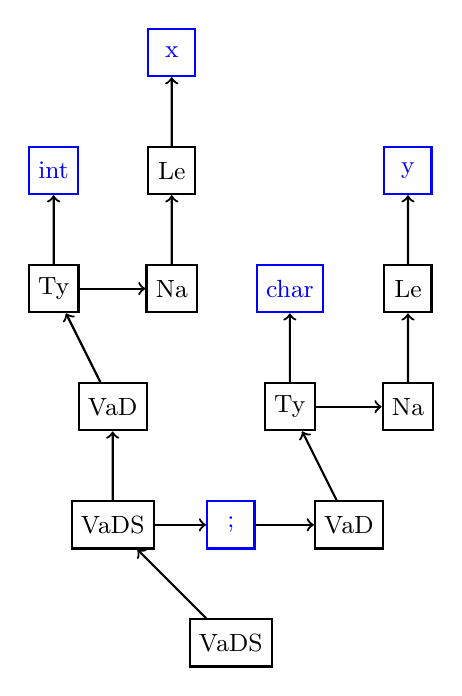
\begin{tikzpicture}
        [font=\small,sibling distance =1.5cm, grow'=up, edge from parent/.style={draw=black, thick,->},
        every node/.style={style A}]

        \node (root) {VaDS}

        child {
            node (VaDS) {VaDS}
            child {
                node (VaD2) {VaD}
                child {
                    node (Ty1) {Ty}
                    child { node[blue] (int) {int} }
                }
                child {
                    node (Na1) {Na}
                    edge from parent[draw=none]
                    child { node (Le1) {Le} child {node[blue] (x) {x} } }
                }
            }
        }
        child {
            node[blue] (sc) {;}
            edge from parent[draw=none]
        }
        child {
            node (VaD1) {VaD}
            edge from parent[draw=none]
            child { node (Ty2) {Ty} child { node[blue] (char) {char}} }
            child {
                node (Na2) {Na}
                edge from parent[draw=none]
                child { node (Le2) {Le} child { node[blue] (y) {y} }}
            }
        };

        \draw[thick, ->] (VaDS)  -- (sc);
        \draw[thick, ->] (sc)    -- (VaD1);
        \draw[thick, ->] (Ty1)   -- (Na1);
        \draw[thick, ->] (Ty2)   -- (Na2);
    \end{tikzpicture}
    \caption{Example subtree}
    \label{fig:example_subtree}
\end{figure}

\subsection{Flattened Sequence}\label{subsec:$fseq$}
The population of symbol tables and subsequent code generation is accomplished by thoroughly parsing the program tree.
Certain grammar tokens have the corresponding sequence element that has the derivation exemplified by
\[XS \to X\ |\ XS; X\]
In the context of symbol definitions, there is $\langle TyDS\rangle, \langle VaDS \rangle$ and $\langle FuDS \rangle$.
To optimize the input for table models, an array of the respective tree elements is preferred over a singular sequence element.
To facilitate this, a method for flattening the sequence is introduced.
\begin{definition}[fseq]
    Let $t = XS$ be a sequence subtree, i.e.
    \[XS \to X \ |\ XS;X\qquad X,XS\in N\]
    Then the flattened sequence of the subtree is given by
    \[fseq(t) = \left[X_1,\dots,X_k\right]\]
    where $k$ is the amount of derived $X$ non-terminals in the tree.
    Algorithm is implemented in the following way:
\end{definition}

\begin{codeblock}[Flattened sequence. Java implementation on \href{https://github.com/fyfsb/dcfg/blob/main/src/main/java/tree/DTE.java}{Github}]
    input: sequence subtree xs,
    output: flattened sequence DTE[]

    fseq(DTE xs) -> DTE[] {
        case xs.label is undefined -> return [];
        case xs.fson.bro is undefined -> [xs.fson];
        otherwise -> fseq(xs.fson) + [xs.fson.bro.bro];
    }
\end{codeblock}
First case is a simple null check, following 2 describe
possible derivations of $xs$:
\begin{itemize}
    \item \verb+xs.fson.bro is undefined+: sequence element derives $XS \to X$. \verb+xs.fson+ is the only
    element in the sequence.
    \item \verb+otherwise+: $xs$ derives $XS \to XS;X$.
    Flattened sequence is recursively obtained for \verb+xs.fson+, to which \verb+xs.fson.bro.bro+ is appended
    (Corresponding to $X$ in the derivation)
\end{itemize}
Working with example from \ref{fig:example_subtree}, we have
\[fseq(VaDS) = [VaD(\verb+int+, \verb+x+), VaD(\verb+char+, \verb+y+)]\]

\subsection{Border Word}\label{subsec:border-word}
Symbol table entries have string values as keys, extracting the name from the respective symbol definition/declaration
requires traversing and concatenating the labels of the leaves of the subtree \verb+<Na>+.
For this purpose, function getting the border word of the subtree is used:
\begin{definition}[bw]
    Let $x \in N \cup T$ be a root for the program subtree.
    Border word of the subtree is given by
    \[
        bw(\verb+x+) = \begin{cases}
                           \verb+x.label.content+&\quad x\in T\\
                           bw(\verb+x.fson+)\circ \bigcirc_{i=1}^k bw(\verb+x.bro+_i)&\quad x\in N
        \end{cases}
    \]
    where $k$ is the number of siblings of \verb+x.fson+\\
    Algorithm:
\end{definition}
\begin{codeblock}[Border word. Java implementation on \href{https://github.com/fyfsb/dcfg/blob/main/src/main/java/tree/DTE.java}{Github}]
    input: derivation tree element x.
    output: concatenated labels of the leaves, string res.

    bw(DTE x) -> string {
        case x is terminal -> return x.label.content;
        otherwise -> {
            res := bw(x.fson);
            for all siblings bro_i of x.fson -> {
                res = res + bw(bro_i);
            }
            return res;
        }
    }
\end{codeblock}

\subsection{Extract Component Pairs}\label{subsec:extract-component-pairs}
The current implementation of the filling of the symbol tables requires extracting the pairs
of form \verb+Ty Na+ (variable declaration) in the string form and performing the lookups in the
type table and the memory struct, respectively.
This step ensures that the context conditions (type being defined, variable name being unique) are satisfied.
We're referring to the aforementioned pattern as a pair component, i.e a pair of tokens $A, B$ derived as
\[ XS \to XS; X\ |\ X\qquad XS,X \in N\qquad A,B\in N\cup T\]
One clear example of such pattern is variable (or parameter) declaration sequence.
\[ VaD \to Ty\ Na\]
Reading the variable declarations occurs at all 3 stages of filling the symbol tables:
\begin{itemize}
    \item Type definitions: reading the components of struct type;
    \item Global variable declarations: consists only of variable declarations;
    \item Function declarations: parameters and local variables.
\end{itemize}
An attempt at simplifying the implementation entails extracting the component pair sequence reads
into the following algorithm:

\begin{definition}[extractCompPairs]
    Let $X \in N$ be a non-terminal deriving a pair
    \[X \to A\ B\]
    where $A,B \in N\cup T$.
    Let $XS \in N$ be a sequence non-terminal deriving
    \[ XS \to XS;X\ |\ X\]
    then extraction of all the component pairs yields the list of tuples of the form
    \[(bw(\verb+A+), bw(\verb+B+)) \]
    We have
    \[ \verb+extrCompPairs(XS)+ = \Bigg[ \Big( bw(fs_1.fson),bw(fs_1.fson.bro) \Big),\dots,\Big( bw(fs_k.fson),bw(fs_k.fson.bro) \Big) \Bigg]\]
    where for $i\in[1:k],\ fs_i \in fseq(xs),\ k=|fseq(xs)|$
\end{definition}
\begin{codeblock}[Extracting component pairs. Java implementation on \href{https://github.com/fyfsb/dcfg/blob/main/src/main/java/tree/DTE.java}{Github}]
    input: DTE xs - sequence element deriving component pairs parent x
    output: string[][] - array of pair border word tuples

    extrCompPairs(DTE xs) -> string[][] {
        fs := fseq(xs)
        result := []
        for all elements fs_i in fs -> {
            case fs_i is separator token (";", ",") -> fs_i = fs_i.bro;

            A := bw(fs_i.fson)
            B := bw(fs_i.fson.bro)

            result.add([A,B])
        }
        return result
    }
\end{codeblock}
Aforementioned function, for the example from Figure~\ref{fig:example_subtree} would return
\[extrCompPairs(VaDS) = [["int", "x"], ["char", "y"]]\]


\section{Filling The Symbol Tables}\label{sec:using-new-tools-for-filling-the-symbol-tables}
In this section, we present a comprehensive overview of the symbol table filling process, leveraging the predefined models and algorithms.
Our approach is guided by the following strategies:
\begin{enumerate}
    \item Type tables:
    \begin{itemize}
        \item Arrays: The array type must be either primitive or defined beforehand.
        Additionally, the array size is validated for correctness, and the new type name should not already exist in the type table.

        \item Structs: Same constraints apply to each component of the structure.
        \item Pointers: It is not required for the pointer target type to be defined previously.
        For that reason, \verb+VarType+ model stores only the name of the target, obtaining the type instance
        requires a lookup in the table.
    \end{itemize}
    \item Global variable tables:
    \begin{itemize}
        \item Variable names should be distinct.
        \item Types should be either primitive, or previously defined.
    \end{itemize}
    \item Function tables:
    \begin{itemize}
        \item Names should be distinct (in this version, we do not account for signatures.
        Thus, function overloading is not allowed).
        \item Return types should be primitive or defined previously.
        \item Parameters and local variables follow the same constraints as global variables.
    \end{itemize}
\end{enumerate}
General overview of the compilation process is shown in Figure~\ref{fig:c0_comp}.
The program tree derives 3 sequence tokens \verb+<TyDS>+, \verb+<VaDS+ and \verb+FuDS+.
Subsequently, the corresponding tables are populated.
Once completed, the body of the main function is extracted from the function table.
For each statement within the main function, assembly code is then generated.
\begin{figure}[h]
    \centering
    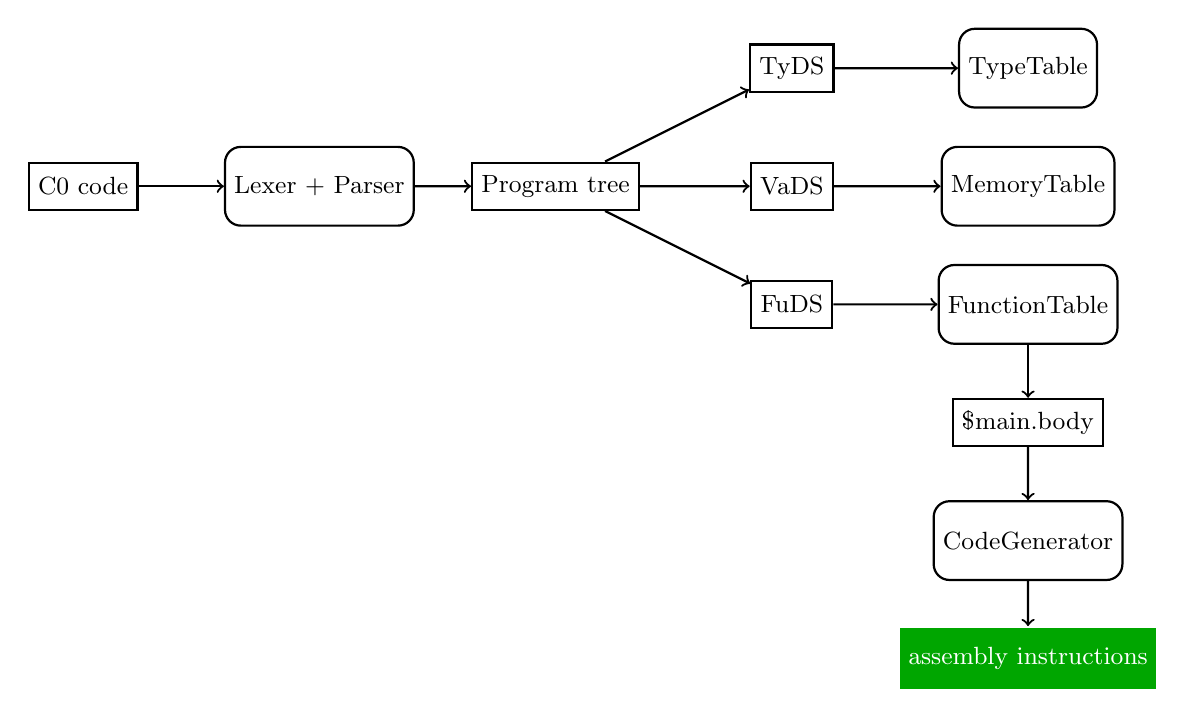
\begin{tikzpicture}
        [font=\small,sibling distance =1.5cm, level distance=3cm, grow'=right, edge from parent/.style={draw=black, thick,->},
        level 4/.style={level distance=3cm},
        level 5/.style={grow'=down, level distance=1.5cm}]


        \node[style A] (root) {C0 code}

        child {
            node[style B] (lp) {Lexer + Parser}
            child {
                node[style A] (pt) {Program tree}
                child {
                    node[style A] (tyds) {TyDS}
                    child {
                        node[style B] (tt) {TypeTable}
                    }
                }
                child {
                    node[style A] (vads) {VaDS}
                    child {
                        node[style B] (mt) {MemoryTable}
                    }
                }
                child {
                    node[style A] (fuds) {FuDS}
                    child {
                        node[style B] (ft) {FunctionTable}
                        child {
                            node[style A] (body) {\$main.body}
                            child {
                                node[style B] (cg) {CodeGenerator}
                                child { node[style C] (ai) {assembly instructions} }
                            }
                        }
                    }
                }
            }
        };

    \end{tikzpicture}\caption{C0 Program Compilation Process}
    \label{fig:c0_comp}
\end{figure}

\subsection{Filling the type table}\label{subsec:filling-the-type-table}
Filling the type table from the \verb+<TyDS>+ token involves flattening the sequence and reading each
type definition separately (Figure~\ref{fig:fill_tt}).
\begin{figure}[h]
    \centering
    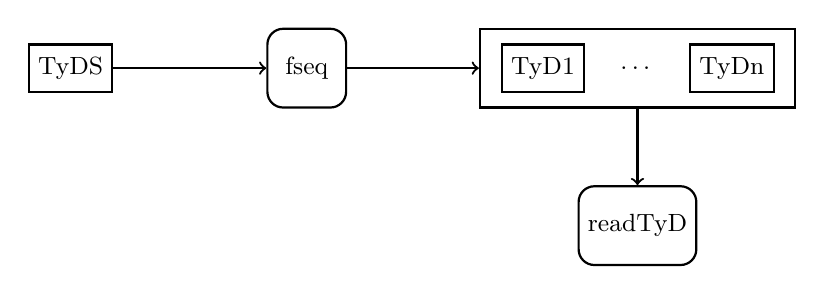
\begin{tikzpicture}
        [font=\small,sibling distance =1.5cm, level distance=3cm, grow'=right, edge from parent/.style={draw=black, thick,->},
        level 3/.style={level distance=1.2cm},
        level 5/.style={grow'=down, level distance=1.5cm}]

        \node[style B]  at (7.2,-2) (readTyD) {readTyD};
        \node[style A, minimum width=4cm, minimum height=1cm] at (7.2, 0) (box) {};
        \node[style A] (tyds) {TyDS}
        child {
            node[style B] (fseq) {\ fseq\ }
            child {
                node[style A] (tyd1) {TyD1} edge from parent[draw=none]
                child {
                    node[draw=none] (dots) {\dots} edge from parent[draw=none]
                    child {
                        node[style A] (tydn) {TyDn} edge from parent[draw=none]
                    }
                }
            }
        };

        \draw[thick, ->] (box)  -- (readTyD);
        \draw[thick, ->] (fseq)  -- (box);
    \end{tikzpicture}\caption{Filling the type table}
    \label{fig:fill_tt}
\end{figure}
\newpage
Each time a derivation tree element is processed, the corresponding pattern matching function ensures
that the passed argument satisfies the required label, as exemplified below.
\begin{codeblock}[fillTypeTable. Java implementation on \href{https://github.com/fyfsb/dcfg/blob/main/src/main/java/table/TypeTable.java}{Github}]
    input: DTE tyds - tree element of type TyDS,
    output: none
    effect: fills the table with new types

    fillTypeTable(DTE tyds) -> void {
        case tyds is not <TyDS> -> error;
        for all element tyD in fseq(tyds) -> readTyD(tyD);
    }
\end{codeblock}
Next step involves implementing \verb+readTyD+.
Given the derivation for \verb+TyD+ tokens, as shown in\\ Figure~\ref{fig:tyd}, uniqueness of the type's name is checked as
\begin{codeblock}
    checkUnique(DTE tyD) {
        nameToken := tyD.fson.bro.bro
        name := bw(nameToken)
        if TypeTable.containsType(name) -> { error }
    }
\end{codeblock}
Subsequently, we perform a case split based on the kind of the
type expression, illustrated in Figure~\ref{fig:readTyD}.
The \verb+struct+ keyword identifies the struct class, the asterisk at the end indicates a pointer, and opening square brackets denote arrays.
These key distinctions are crucial, as the actual implementation (unlike the representation in Figure~\ref{fig:readTyD}) relies on pattern matching solely based on these differences.
Consequently, visiting the first two children of the type expression subtree is sufficient.
\begin{figure}[h]
    \centering
    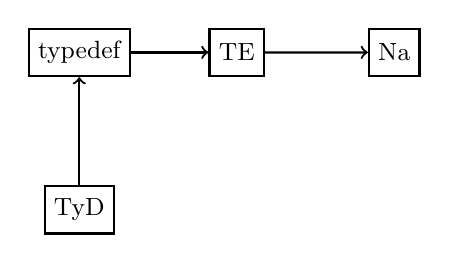
\begin{tikzpicture}
        [font=\small, level distance=2cm, grow'=up, edge from parent/.style={draw=black, thick,->},
        level 2/.style={grow'=right}]

        \node[style A] (tyd) {TyD}
        child {
            node[style A] (td) {typedef}
            child {
                node[style A] (te) {TE}
                child { node[style A] (na) {Na} }
            }
        };

    \end{tikzpicture}\caption{Derivation of the type definition}
    \label{fig:tyd}
\end{figure}

\begin{figure}[h]
    \centering
    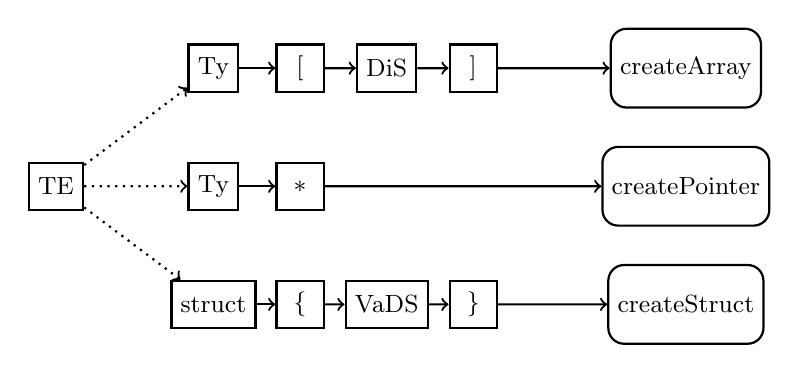
\begin{tikzpicture}
        [font=\small, level distance=2cm, grow'=right, edge from parent/.style={draw=black, thick,->},
        level 2/.style={grow'=right, level distance=1.1cm}]

        \node[style B]  at (8,1.5) (createArray) {createArray};
        \node[style B]  at (8,0) (createPointer) {createPointer};
        \node[style B]  at (8,-1.5) (createStruct) {createStruct};

        \node[style A] (te) {TE}
        child {
            node[style A] (ty1) {Ty} edge from parent[draw=none]
            child {
                node[style A] (lb) {[}
                child {
                    node[style A] (dis) {DiS}
                    child {
                        node[style A] (rb) {]}
                    }
                }
            }
        }
        child {
            node[style A] (ty2) {Ty} edge from parent[draw=none]
            child { node[style A] (ptr) {$*$} }
        }
        child {
            node[style A] (struct) {struct} edge from parent[draw=none]
            child {
                node[style A] (lcb) {\{}
                child {
                    node[style A] (vads) {VaDS}
                    child { node[style A] (rcb) {\}} }
                }
            }
        };

        \draw[thick, ->] (rb)  -- (createArray);
        \draw[thick, ->] (ptr)  -- (createPointer);
        \draw[thick, ->] (rcb)  -- (createStruct);


        \draw[dotted,thick, ->] (te)  -- (ty1);
        \draw[dotted,thick, ->] (te)  -- (ty2);
        \draw[dotted,thick, ->] (te)  -- (struct);
    \end{tikzpicture}\caption{Reading the type definition}
    \label{fig:readTyD}
\end{figure}

\newpage

\subsubsection{Adding array type}
Figure~\ref{fig:addArray} illustrates the process of adding an array type to the type table.
Initially, the \verb+<Ty>+ type is checked for being primitive or defined previously.
This is achieved by extracting the type name from the border word of the type token and searching for the corresponding \verb+VarType+ entry in the type table.
\begin{codeblock}
    checkDefined(DTE ty) -> bool {
        name := bw(ty)
        return TypeTable.containsType(ty)
    }
\end{codeblock}
The subsequent step involves verifying the non-negativity of array's length.
Any failure in these checks results in an error.
Upon passing the check, the array's target type is obtained from the corresponding entry in the type table.
The array's size is extracted from the parsed \verb+<DiS>+ token, and name is the border word of \verb+<Na>+.
The resulting record is then added to the type table.

\begin{figure}[h]
    \centering
    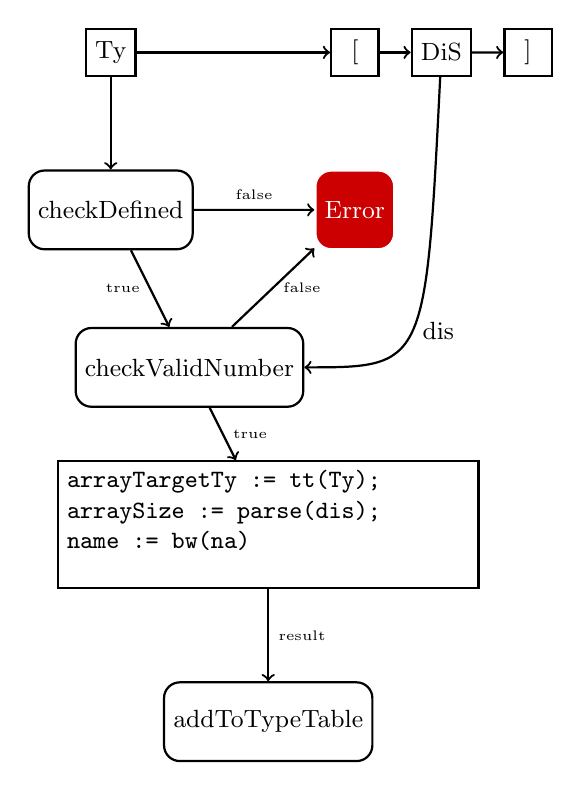
\begin{tikzpicture}
        [font=\small, level distance=3.1cm, grow'=right, edge from parent/.style={draw=black, thick,->},
        level 2/.style={grow'=right, level distance=1.1cm}]

        \node[style B] at (2, -8.5) (addToTT) {addToTypeTable};
        \node[style A] at (2, -6) (done) {
            \begin{minipage}{5cm}
                \begin{verbatim}arrayTargetTy := tt(Ty);
arraySize := parse(dis);
name := bw(na)
                \end{verbatim}
            \end{minipage}
        };
        \node[style B] at (1,-4) (valid) {checkValidNumber};
        \node[style B] at (0, -2) (defined) {checkDefined}
        child { node[style D] (err) {Error} edge from parent  [->] node [above] {\tiny false}};
        \node[style A] (ty1) {Ty}
        child {
            node[style A] (lb) {[}
            child {
                node[style A] (dis) {DiS}
                child {
                    node[style A] (rb) {]}
                }
            }
        };
        \draw[thick, ->] (ty1) -- (defined);
        \draw[thick, ->] (defined) -- node[midway, left] {\tiny true} (valid);
        \draw[thick, ->] (valid) -- node[midway, right] {\tiny false} (err);
        \draw[thick, ->] (dis) .. controls (4,-4) .. node[midway, right] {dis} (valid);
        \draw[thick, ->] (valid) -- node[right] {\tiny true} (done);
        \draw[thick, ->] (done) -- node[right] {\tiny result} (addToTT);
    \end{tikzpicture}\caption{Adding array type}
    \label{fig:addArray}
\end{figure}
\newpage

\subsubsection{Adding Pointer Type}
As described in the beginning, strategy for adding the pointers doesn't require the target type to be defined
previously, thus possibly resulting in a NULL-type pointer (initially).
Actual access for the target type involves lookups in the type table:
\begin{codeblock}
    getPointerTargetType() -> VarType {
        type := TypeTable.getTypeOrNull(ptrTargetTyName)
        if type == null -> { error }
        return type
    }
\end{codeblock}
\begin{figure}[h]
    \centering
    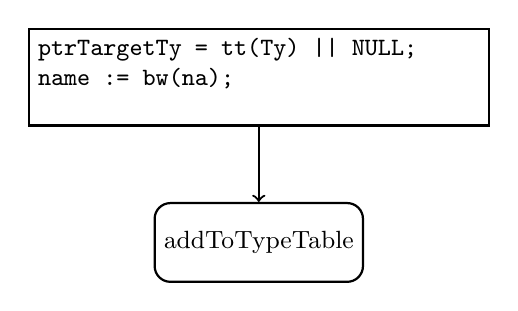
\begin{tikzpicture}
        [font=\small, level distance=2.1cm, grow'=down, edge from parent/.style={draw=black, thick,->},]
        \node[style A] (done) {
            \begin{minipage}{5.5cm}
                \begin{verbatim}ptrTargetTy = tt(Ty) || NULL;
name := bw(na);
                \end{verbatim}
            \end{minipage}
        }
        child { node[style B] {addToTypeTable}};
    \end{tikzpicture}\caption{Adding pointer type}
    \label{fig:addPointer}
\end{figure}

\subsubsection{Adding Struct type}
In Figure~\ref{fig:addStruct}, the checking process for structs components is illustrated.
Similar to arrays, the type being primitive or defined previously is verified using the same checker function.
However, uniqueness of the names is required within the components.
To address this, a set is initialized and updated within the loop.
Additionally, inside the loop, displacement is accumulated, satisfying the formula
\[ displ(comp_i, struct) = ba(struct) + \sum_{j=0}^{i-1}size(comp_j)\]
At the end of the loop, the displacement variable represents the sum of the sizes of all components,
equivalent to the size of the entire struct, which is then assigned to the respective attribute.
After passing the name, size and components to the struct type builder, new instance of the \verb+VarType+
is added to the type table.
\begin{codeblock}[Adding struct type. Java implementation on \href{https://github.com/fyfsb/dcfg/blob/main/src/main/java/table/TypeTable.java}{Github}]
    ...
    components := fseq(VaDS)
    compNames := emptySet()
    strComps := Map<String, Variable>()
    displacement := 0
    for all comp in components -> {
        ty := comp.fson
        na := comp.fson.bro

        checkDefined(ty)
        if compNames.contains(na) -> { error }
        compNames.add(na)

        type := TypeTable.getType(bw(ty))
        strComps.put(na, new Variable(na, 0, type, displacement))
        displacement += size(type)
    }
    structType := structBuilder
        .setName(bw(Na))
        .setSize(displacement)
        .setComps(strComps).build()
    TypeTable.addType(structType)
\end{codeblock}
\begin{figure}[h]
    \centering
    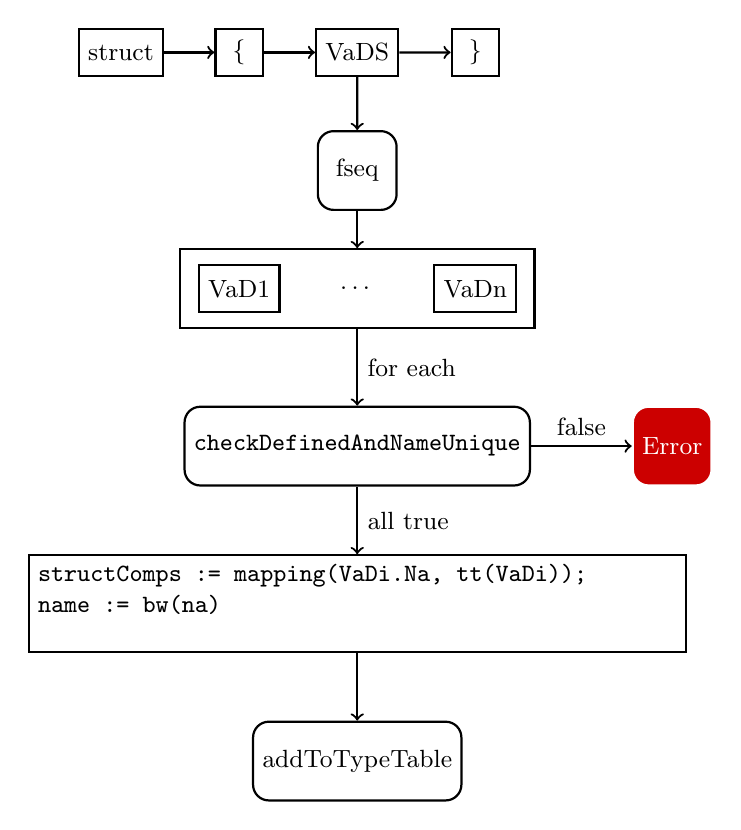
\begin{tikzpicture}
        [font=\small, level distance=1.5cm, grow'=right, edge from parent/.style={draw=black, thick,->},
        level 2/.style={grow'=right, level distance=1.5cm}]

        \node[style B] at (3,-9) (addToTT) {addToTypeTable};
        \node[style A] at (3,-7) (code) {
            \begin{minipage}{8cm}
                \begin{verbatim}structComps := mapping(VaDi.Na, tt(VaDi));
name := bw(na)
                \end{verbatim}
            \end{minipage}
        };
        \node[style D] at (7, -5) (err) {Error};
        \node[style B] at (3, -5) (check) {\verb+checkDefinedAndNameUnique+};
        \node[style A, minimum width=4.5cm, minimum height=1cm] at (3, -3) (box) {};
        \node[style A] at (1.5,-3) (vad1) {VaD1}
        child {
            node[draw=none] (dots) {$\dots$} edge from parent[draw=none]
            child { node[style A] (vadn) {VaDn} edge from parent[draw=none]}
        };
        \node[style B] at (3,-1.5) (fseq) {fseq};
        \node[style A] (struct) {struct}
        child {
            node[style A] (lcb) {\{}
            child {
                node[style A] (vads) {VaDS}
                child { node[style A] (rcb) {\}} }
            }
        };

        \draw[thick, ->] (vads) -- (fseq);
        \draw[thick, ->] (fseq) -- (box);
        \draw[thick, ->] (box) -- node[midway, right] {for each} (check);
        \draw[thick, ->] (check) -- node[midway, above] {false} (err);
        \draw[thick, ->] (check) -- node[midway, right] {all true} (code);
        \draw[thick, ->] (code) -- (addToTT);
    \end{tikzpicture}\caption{Adding Struct type}
    \label{fig:addStruct}
\end{figure}
\newpage

\subsection{Filling memory table}\label{subsec:filling-memory-table}
Since variable scopes are decided to be stored inside a struct, we treat global
variable declaration sequence \textbf{almost} as a type definition of form:

\begin{codeblock}
typedef struct { VaDS } $gm;
\end{codeblock}
Single difference from a regular type definition is, that the newly created type
is not added to the type table, otherwise the following code would be a valid C0 program:
\begin{codeblock}
int a;
bool b;
char c;
int main() {
    $gm k;
    ...
    k.b = true;
    return k.a
}
\end{codeblock}
Therefore, we're employing the modified function for adding the struct types:
\newpage
\begin{codeblock}
...
structType := structBuilder.setName(bw(Na)).setSize(displacement).setComps(strComps).build()
return structType // just creating and returning, without adding to the type table
\end{codeblock}
\subsection{Filling the function table}
Approach is similar to the type tables, as shown in Figure~\ref{fig:fillFT}, function definitions are flattened and
read separately.
\begin{figure}[h]
\centering
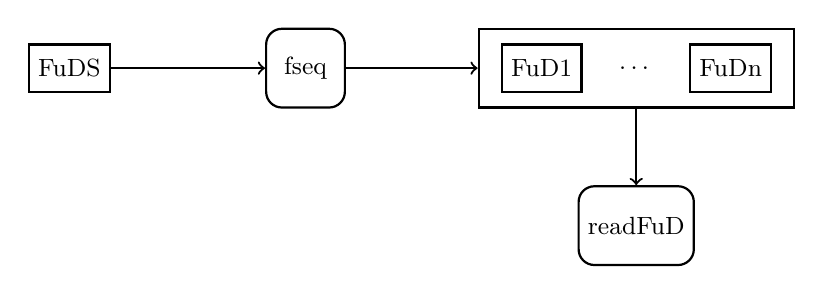
\begin{tikzpicture}
[font=\small,sibling distance =1.5cm, level distance=3cm, grow'=right, edge from parent/.style={draw=black, thick,->},
level 3/.style={level distance=1.2cm},
level 5/.style={grow'=down, level distance=1.5cm}]

\node[style B]  at (7.2,-2) (readTyD) {readFuD};
\node[style A, minimum width=4cm, minimum height=1cm] at (7.2, 0) (box) {};
\node[style A] (tyds) {FuDS}
child {
node[style B] (fseq) {\ fseq\ }
child {
node[style A] (tyd1) {FuD1} edge from parent[draw=none]
child {
node[draw=none] (dots) {\dots} edge from parent[draw=none]
child {
node[style A] (tydn) {FuDn} edge from parent[draw=none]
}
}
}
};

\draw[thick, ->] (box)  -- (readTyD);
\draw[thick, ->] (fseq)  -- (box);
\end{tikzpicture}
\caption{Filling the function table}
\label{fig:fillFT}
\end{figure}

As in the previous parts, type is verified to be either primitive or defined previously. Upon success, return
type is stored:
\begin{codeblock}
ty := bw(Ty)
checkDefined(ty)
returnType = TypeTable.getType(ty)
\end{codeblock}
function name is checked for uniqueness and the respective attribute assigned:
\begin{codeblock}
na := bw(Na)
if FunctionTable.containsFunction(na) -> { error }
name := na
\end{codeblock}
A local memory struct is generated by merging the sequences of parameters and local variables.
Initially, the number of parameters is stored. As shown in Figure~\ref{fig:readFuD},
\verb+<PaDS>+ and \verb+<VaDS>+ are flattened and combined into a single list. Under the hood, component pairs
are extracted and forwarded to the struct builder (Utilizing the builder pattern for constructing \verb+VarType+ instances,
the project's source code provides a reference for this implementation).
\begin{codeblock}
componentPairs := extractCompPairs(PaDS)
componentPairs.addAll(extractCompPairs(VaDS))
structBuilder.setCompPairs(componentPairs)
... // same logic follows, as in creation of the global memory struct
\end{codeblock}
\begin{figure}[h]
\centering
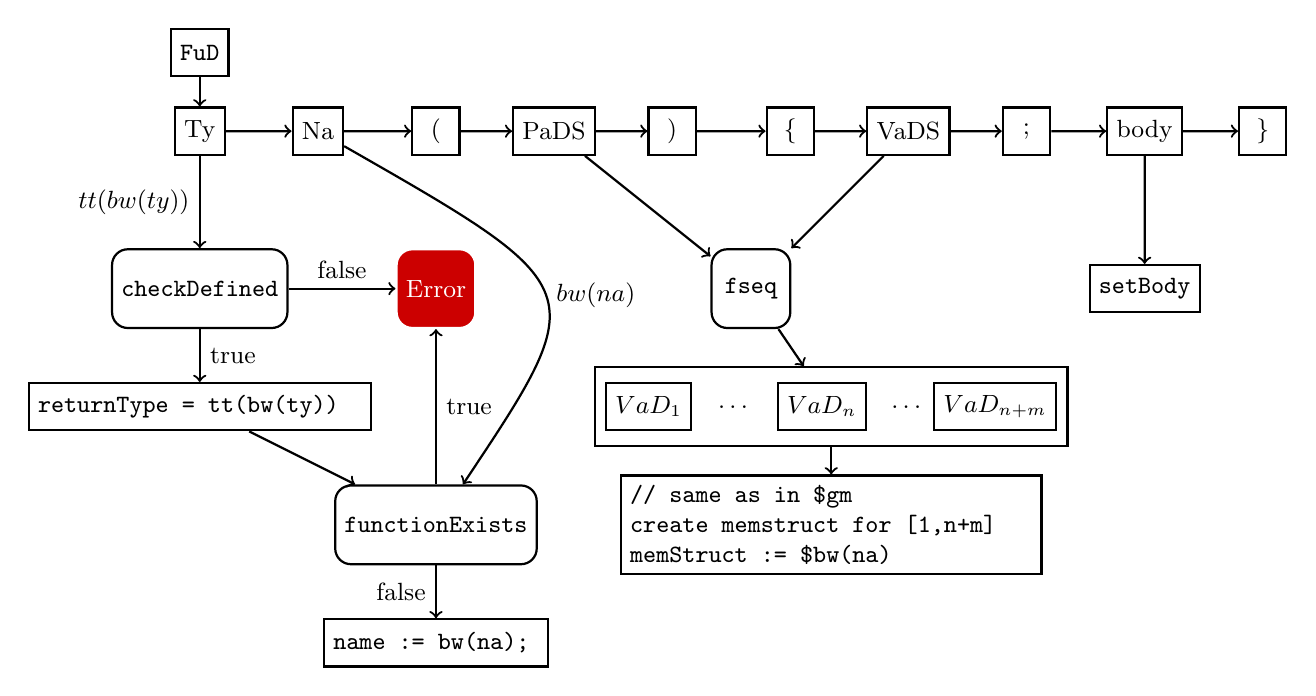
\begin{tikzpicture}
[font=\small,sibling distance =1.5cm, level distance=1.5cm, grow'=right, edge from parent/.style={draw=black, thick,->}]

\node[style A] at (12, -3) (addbody) {\verb+setBody+};
\node[style A] at (8.02, -6) (struct) {
\begin{minipage}{5cm}
\begin{verbatim}
// same as in $gm
create memstruct for [1,n+m]
memStruct := $bw(na)
\end{verbatim}
\end{minipage}
};
\node[style A, minimum width=6cm, minimum height=1cm] at (8.02, -4.5) (box) {};
\node[style A] at (5.7,-4.5) (vad1) {$VaD_1$};
\node[draw=none] at (6.8, -4.5) (dots1) {$\dots$};
\node[style A] at (7.9,-4.5) (vadn) {$VaD_n$};
\node[draw=none] at (9, -4.5) (dots2) {$\dots$};
\node[style A] at (10.1,-4.5) (vadnm) {$VaD_{n+m}$};
\node[style B] at (7, -3) (fseq) {\verb+fseq+};
\node[style A] at (3, -7.5) (nameCode) {
\begin{minipage}{2.5cm}
\begin{verbatim}
name := bw(na);
\end{verbatim}
\end{minipage}
};
\node[style B] at (3, -6) (functionExists) {\verb+functionExists+};
\node[style A] at (0, -4.5) (checkCode) {
\begin{minipage}{4cm}
\begin{verbatim}
returnType = tt(bw(ty))
\end{verbatim}
\end{minipage}
};
\node[style D] at (3, -3) (err)    {Error};
\node[style B] at (0, -3) (check) {\verb+checkDefined+};
\node[style A] (fud) {\verb+FuD+};
\node[style A] at (0, -1) (ty) {Ty}
child {
node[style A] (na) {Na}
child {
node[style A] (lp) {(}
child {
node[style A] (pads) {PaDS}
child {
node[style A] (rp) {)}
child {
node[style A] (lcb) {\{}
child {
node[style A] (vads) {VaDS}
child {
node[style A] (sc) {;}
child {
node[style A] (body) {body}
child{
node[style A] (rcb) {\}}
}
}
}
}
}
}
}
}
};
\draw[thick, ->] (fud) -- (ty);
\draw[thick, ->] (ty) -- node[midway, left] {$tt(bw(ty))$} (check);
\draw[thick, ->] (check) -- node[midway, above] {false} (err);
\draw[thick, ->] (check) -- node[midway, right] {true} (checkCode);
\draw[thick, ->] (checkCode) -- (functionExists);
\draw[thick, ->] (na) .. controls (5, -3) .. node[midway,right] {$bw(na)$} (functionExists);
\draw[thick, ->] (functionExists) -- node[midway, right] {true} (err);
\draw[thick, ->] (functionExists) -- node[midway, left] {false} (nameCode);
\draw[thick, ->] (pads) -- (fseq);
\draw[thick, ->] (vads) -- (fseq);
\draw[thick, ->] (fseq) -- (box);
\draw[thick, ->] (box) -- (struct);
\draw[thick, ->] (body) -- (addbody);
\end{tikzpicture}
\caption{Reading function definition}
\label{fig:readFuD}
\end{figure}
In the final step, a new function entry is added to the table. With the symbol tables now filled, we proceed to the implementation
of code generation.

\section{Helper Components for Code Generation}\label{sec:helpers}
In the upcoming section, we lay the groundwork for our code generation process by introducing crucial
helper components. Among these, we delve into the assignment of registers using pebble game. Furthermore, we
introduce the \verb+FunctionCall+ class, designed to streamline the management of function calls. This class stores
essential information such as the function, recursion depth, and displacement from the base pointer. Besides the practical
purpose, \verb+FunctionCall+ enables convenient debugging. Additionally, the \verb+Configuration+ class is implemented, that
not only manages the stack of function calls, but also provides access to the current function and incorporates the pebble game
logic, including acquiring free registers and releasing them when needed. Finally, we introduce new record \verb+VarReg+, which is
simply a data class containing the variable, type and the register. Later on, storing the register inside a record enables
dividing the code generation parts by context and allows working with repeating patterns recursively.
\subsection{Register Distribution}
Referencing the Sethi-Ulman algorithm described in the system architecture book \cite{sysbook}, Section 12.2.1, we align the pebble game moves with the state of registers in the statement,
as outlined below:
\begin{itemize}
    \item A register is considered occupied when a pebble is placed on a corresponding node.
    \item Moving the pebble doesn't alter the number of free registers, an occupied register is retained.
    \item Removing the pebble from the node releases the associated register, rendering it available.
    \item All registers are freed in the end of the statement.
\end{itemize}
Therefore, a register is assigned for the expression node, it is released either when the statement is completed, or after
the binary operation if the respective pebble, associated with one of the operands, is removed from the node, i.e. is not
storing the result of the operation. Given that, we're choosing an approach different from the pebble game, by which evaluation of
the expressions by the induction over the trees (quoting \cite{sysbook} Section 12.2.1) is preserved (detailed description of code generation
of the expressions can be found in Section \ref{subsec:generating_assignments}). However, register states are
maintained globally by a dedicated class. The main idea is to keep track of the occupied registers, release the single register corresponding to the binary operation's right operand, after the operation's finished,
and release every register after each statement.
\subsubsection{Keeping the track of the occupied registers with a single pointer}
Key idea is to employ a straightforward pointer to the first available register, occupying the register entails increasing the pointer,
releasing triggers the decrement.
\begin{codeblock}
int registerPointer := 1; // first free register

getFreeReg() -> int {
    if registerPointer >= MAX_AVAILABLE -> { error }
    registerPointer := registerPointer + 1
    return registerPointer - 1
}

releaseReg() {
    registerPointer = min(1, registerPointer - 1)
}
\end{codeblock}
Although this implementation satisfies the current grammar, the naive approach does not work for the extended grammar
with inline assembly portions:
\begin{codeblock}[Inline assembly]
gpr(j) = e { 4, 6 };
e = gpr(j) { 2, 7 };
// Here, e is an expression
\end{codeblock}

The aforementioned listing is an example of the inline assembly statements of C0. The sets of numbers right after the assignments
specify the registers which are restricted to be changed during the respective assignment. Although,
simple repeated incrementing of the register pointer will work while evaluating inline assembly statements, although releasing the
registers will result in a single decrement, leaving out a range of available registers out of scope.

\subsubsection{Distributing Registers With Boolean Arrays}
Workaround is to use a boolean array, with each item indicating the availability of the register
with the respective index. Getting the register becomes an operation of getting first one and setting zero,
releasing - setting one. This approach works for inline assembly portions as well, since it suffices to make
each register from set \verb+J+ unavailable during the statement.
\newpage
\begin{codeblock}[Pebble game]
registers = new boolean[MAX_AVAILABLE];
...
int reg = f1(registers); // getting first one
registers[reg - 1] = false; // occupying while in use
...
registers[reg - 1] = true; // releasing the register
\end{codeblock}
\subsection{Configuration Class}
It is important to keep track of the current function (for variable binding). For debugging, it's also helpful to
store the recursion depth and the displacement of each call. We define a record for this purpose
\begin{codeblock}[Function call. Java implementation on \href{https://github.com/fyfsb/dcfg/blob/main/src/main/java/config/FunctionCall.java}{Github}]
class FunctionCall {
    Fun function;
    int rd;
    int displacement; // from bpt
}
\end{codeblock}
We're combining the function call stack and pebble game logic into Configuration class.
\begin{codeblock}[Configuration class. Java implementation on \href{https://github.com/fyfsb/dcfg/blob/main/src/main/java/config/Configuration.java}{Github}]
class Configuration {
    boolean[] registers; // for pebble game
    Stack<FunctionCall> stack;

    Fun currentFunction () { ... }
    void pop() { ... }
    int getRegister() { ... }
    void freeRegister(int reg) { ... }
}
\end{codeblock}

\subsection{VarReg}
Considering the tree structure of the program, it is convenient to employ recursive traversal algorithms in the code generation.
Moreover, by itself, code generation entails only adding the handler functions for the respective tree patterns. However, this
approach needs to be integrated with the current implementation of the pebble game and it's vital
to keep track of the registers of the corresponding values. For that purpose, we add one more class:
\begin{codeblock}[VarReg class. Java implementation on \href{https://github.com/fyfsb/dcfg/blob/main/src/main/java/model/VarReg.java}{Github}]
class VarReg {
    Variable var;
    int reg;
    VarType type;
}
\end{codeblock}
The \verb+VarReg+ class is the main data structure for generating the assembly instructions.
It stores the reference to the variable, for \verb+<id>+ bindings, type for ensuring the type safety and the register
assigned from the pebble game and used in the assembly instruction.
\verb+Variable+ and \verb+VarType+ are separated. When dealing with \verb+<id>+ bindings, the respective variable is
extracted from the struct and \verb+type = var.type+. Other case is handling constants, for that the respective
type is set
\begin{itemize}
\item \verb+<CC>+ - \verb+CHAR+
\item \verb+<C>+ - \verb+INT+ or \verb+UINT+
\item \verb+<BC>+ - \verb+BOOL+
\end{itemize}
and the variable attribute is set to \verb+null+. You can find the usages of the \verb+VarReg+ class
described in the Section \ref{sec:code_gen}

\section{Code Generation}\label{sec:code_gen}
In this section, using the data structures defined so far, we introduce the classes responsible for the code generation, and describe the handler
functions for each pattern. For simplicity, classes are grouped by the context and purpose. Here, we refer to these structures as
\verb+Evaluator/Helper+ classes. Having almost all methods static, these classes encapsulate nothing except the generated instruction list.
Evaluators' methods are the direct adaptations of the program translation rules described in the system architecture book
\cite{sysbook}, Sections 12.2-12.4. We have
\subsection{ConstEvaluator}
This class generates instructions for \verb+<C>+, \verb+<BC>+ and \verb+<CC>+:
\begin{codeblock}[Constant Evaluator. Java implementation on \href{https://github.com/fyfsb/dcfg/blob/main/src/main/java/codegen/ConstantEvaluator.java}{Github}]
class ConstEvaluator {
    evaluateNumberConstant(DTE c) -> VarReg {
        assert c is <C>

        reg := Configuration.getFreeReg()
        value := parse(c)
        type := if c ends with 'u' then UINT else INT

        case type == UINT -> {
            add new instruction [ addi $reg $reg value ]
        }

        otherwise -> {
            add new instruction [ addiu $reg $reg value ]
        }

        return new VarReg(reg, type)
    }

    evaluateBooleanConstant(DTE bc) -> VarReg {
        assert bc is <BC>
        reg := Configuration.getFreeReg()
        word := bw(bc)

        value = if word == 'true' then 1 else 0
        add new instruction [ addi $reg $reg value]
        return new VarReg(reg, BOOL)
    }

    evaluateCharConstant(DTE cc) -> VarReg {
        assert cc is <CC>
        reg := Configuration.getFreeReg()
        value := parse(cc)
        add new instruction [ addi $reg $reg value ]
        return new VarReg(reg, CHAR)
    }
}
\end{codeblock}
\subsection{Expression Evaluator}
Generates instructions for arithmetic and boolean expressions, i.e. \verb+<E>+ and \verb+<BE>+.
Implementation is described later in the section.
\begin{codeblock}[ExpressionEvaluator. Java implementation on \href{https://github.com/fyfsb/dcfg/blob/main/src/main/java/codegen/ExpressionEvaluator.java}{Github}]
class ExpressionEvaluator {
    // input <E>
    evaluateArithmeticExpression(DTE e) -> VarReg { ... }

    // input <BE>
    evaluateBooleanExpression(DTE be) -> VarReg { ... }

    // Straightforward case split on 'op'
    evaluateBinaryOperation(VarReg left, DTE op, VarReg right) -> VarReg { ... }

    // input <Atom>
    evaluateAtom(DTE atom) -> VarReg { ... }
}
\end{codeblock}

\subsection{Id Evaluator}
Binds and evaluates the variables (\verb+<id>+). The method \verb+evaluateId+ gets passed the \verb+<id>+ token,
whereas \verb+bindVariableName+ binds the \verb+bw(Na)+ to the respective memory struct, and generates the code for
calculating the base address of the variable. Depending on the R-label (system architecture book \cite{sysbook}, Section 12.2.2),
\verb+evaluateId+ returns the left or right value of the expressions (which differ by the single dereference). Here, we utilize
the \verb+lv: bool+ (left value) parameter satisfying $lv = \neg R$. The detailed review of the implementation can be found in the Section \ref{subsec:generating_assignments}.
\newpage
\begin{codeblock}[IdEvaluator. Java implementation on \href{https://github.com/fyfsb/dcfg/blob/main/src/main/java/codegen/IdEvaluator.java}{Github}]
class IdEvaluator {
    evaluateId(DTE id) -> VarReg { ... }
    bindVariableName(DTE na) -> VarReg { ... }
}
\end{codeblock}
\subsection{Memory Helper}
Contains the logic for increasing/decreasing stack and heap pointers. This class is used in the allocations and function calls.
\begin{codeblock}[MemoryHelper. Java implementation on \href{https://github.com/fyfsb/dcfg/blob/main/src/main/java/codegen/MemoryHelper.java}{Github}]
class MemoryHelper {
    increaseHeapPointer(int size) { ... }
    increaseStackPointer(int size) { ... }
}
\end{codeblock}
\subsection{Code Generator}
Gets passed the initial program, encapsulates the generated instructions, delegates tree patterns to other
evaluator classes. Directly manages function calls, conditional and loop statements.

\begin{codeblock}[Code Generator. Java implementation on \href{https://github.com/fyfsb/dcfg/blob/main/src/main/java/codegen/CodeGenerator.java}{Github}]
class CodeGenerator {
    generateCodeForFunctionCall(FunctionCall call) {
        function := call.function
        if !FunctionTable.containsFunction(function) -> { error }

        // any function other than 'main'
        if call.rds is defined -> {
            reg := Configuration.getFreeReg()
            add new instructions [
                addi $reg $0 -(size(function) - 4),
                addi $RA $reg 0
            ]
            Configuration.freeRegister(reg) // release
        }

        // body -> RSt | StS ; RSt
        case function.body.fson is <body> -> generateRSt(body.fson, call)
        otherwise -> {
            generateStS(body.fson)
            generateRSt(body.fson.bro.bro, call)
        }
    }

    generateStS(DTE sts) {
        for all st in fseq(sts) -> {
            generateSt(st)
            Configuration.freeAllRegisters()
        }
    }

    ...
}
\end{codeblock}
As can be seen in \verb+CodeGenerator+, starting the compilation process entails creating a function call for
\verb+main+ function and forwarding it to \verb+CodeGenerator.generateCodeForFunctionCall+ method:
\begin{codeblock}
if !FunctionTable.containsFunction("main") -> { halt } // we are done

mainFunction := FunctionTable.getFunction("main")
mainCall := Configuration.createFunctionCall(mainFunction)

CodeGenerator.generateCodeForFunctionCall(mainCall)
\end{codeblock}
The method checks if the result destination is defined (for any function other than main it will be defined
and contain the pointer to the base address of the variable the result gets assigned to). In such case, the return address
register gets assigned the base address of the result destination variable. Subsequently, methods generating code for
statements are called.

\subsection{Generating for Statements}
To generate code for statements, a case split is performed based on statement types, as depicted in Figure~\ref{fig:st_types}.
Three distinct patterns are identified:
\begin{itemize}
    \item Assignments: Statements commencing with and identifier followed by an assignment operator.
    \item Loops: Statements beginning with the \verb+while+ keyword.
    \item Conditionals: Statements initiated with the \verb+if+ keyword.
\end{itemize}

\begin{figure}[h]
\centering
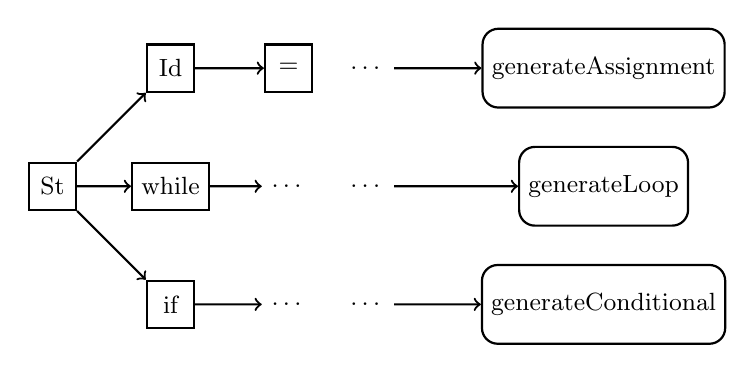
\begin{tikzpicture}
[font=\small,sibling distance =1.5cm, level distance=1.5cm, grow'=right, edge from parent/.style={draw=black, thick,->},
level 3/.style={level distance=1cm},
level 4/.style={level distance=3cm}]

\node [style A] (st) {St}
child {
node [style A] (id) {Id}
child {
node [style A] (eq) {=}
child { node[draw=none] (dots) {$\dots$} edge from parent[draw=none]
child { node[style B] (assignment) {generateAssignment}}
}
}
}
child {
node [style A] (while) {while}
child {
node [draw=none] (eq) {$\dots$}
child { node[draw=none] (dots) {$\dots$} edge from parent[draw=none]
child { node[style B] (loop) {generateLoop}}
}
}
}
child {
node [style A] (if) {if}
child {
node [draw=none] (eq) {$\dots$}
child { node[draw=none] (dots) {$\dots$} edge from parent[draw=none]
child {node[style B] (conditional) {generateConditional}}}
}
};

\end{tikzpicture}
\caption{Statement types}
\label{fig:st_types}
\end{figure}
\newpage
\subsection{Generating Assignments}\label{subsec:generating_assignments}
As illustrated in Figure~\ref{fig:gen_assignment}, the evaluation of an identifier involves storing the left value of the corresponding variable inside a register,
returned within the \verb_VarReg_ record instance \verb+verRegId+.
On the other hand, the assigned value (\verb+X+) is also evaluated, and its right value is stored in the register associated with \verb+varRegValue+.
Both instances of \verb+VarReg+ contain the types of the variables, and a verification is conducted to ensure their equality.
In case of a mismatch, a type safety error is raised; otherwise, the assignment is concluded with a store instruction.
\begin{figure}[h]
\centering
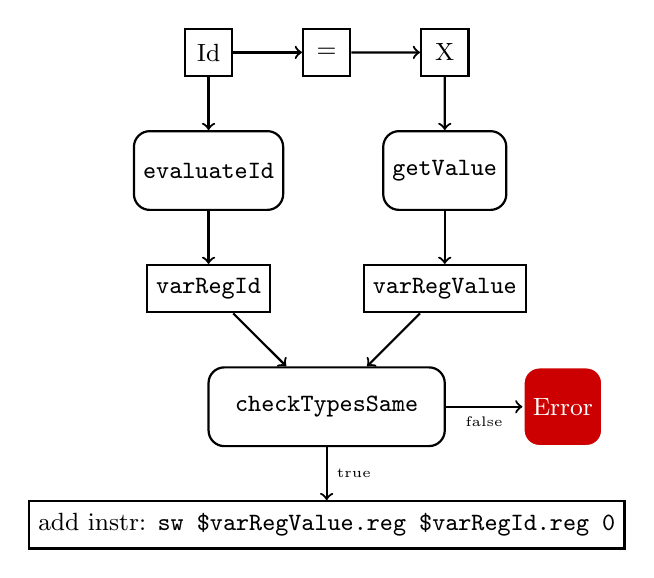
\begin{tikzpicture}
[font=\small,sibling distance =1.5cm, level distance=1.5cm, grow'=right, edge from parent/.style={draw=black, thick,->}]
\node[style A] (id) {Id}
child {
node [style A] (eq) {=} child { node[style A] (x) {X}}
};

\node[style B] at (0, -1.5) (evaluateId) {\verb+evaluateId+};
\node[style A] at (0, -3) (varRegId) {\verb+varRegId+};
\node[style B] at (3, -1.5) (getValue) {\verb+getValue+};
\node[style A] at (3, -3) (varRegValue) {\verb+varRegValue+};
\node[style B, minimum width=3cm] at (1.5, -4.5) (check) {\verb+checkTypesSame+};
\node[style D] at (4.5, -4.5) (error) {Error};
\node[style A] at (1.5, -6) (instr) {add instr: \verb+sw $varRegValue.reg $varRegId.reg 0+};

\draw[thick, ->] (id) -- (evaluateId);
\draw[thick, ->] (x) -- (getValue);
\draw[thick, ->] (evaluateId) -- (varRegId);
\draw[thick, ->] (getValue) -- (varRegValue);
\draw[thick, ->] (varRegId) -- (check);
\draw[thick, ->] (varRegValue) -- (check);
\draw[thick, ->] (check) -- node[midway, below] {\tiny false} (error);
\draw[thick, ->] (check) -- node[midway, right] {\tiny true} (instr);
\end{tikzpicture}
\caption{Generate Assignment}
\label{fig:gen_assignment}
\end{figure}

The evaluation of the identifier, as shown in the listing below, receives the
\verb+<id>+ token and a boolean parameter \verb+lv+, indicating the left value.
When \verb+lv=false+, the right value of the identifier is needed.
Upon computing the base address, an additional dereference is appended to the instruction list.
Otherwise, no extra dereference is added. Regardless of the \verb+lv+ parameter, if identifier
derives the usage of 'address-of' operator, extra dereference is omitted. Base address of the variable
is bound by the call of \verb+bindVariable+ from class \verb+IdEvaluator+.

\begin{figure}[h]
\centering
\begin{codeblock}[evaluateId. Java implementation on \href{https://github.com/fyfsb/dcfg/blob/main/src/main/java/codegen/IdEvaluator.java}{Github}]
input: DTE id, bool lv (checks if additional dereference is required)
output: VarReg result - bound identificator

evaluateId(DTE id, bool lv) -> VarReg {
    res := bindVariable(id)
    if (id.children is not <id>& and !lv) {
        add new instruction [lw $res.reg $res.reg 0] // dereference
    }
    return res
}
\end{codeblock}
\label{fig:evalId}
\end{figure}

\newpage
Binding the variable based on the pattern:
\begin{itemize}
\item \verb+<Na>+: Name is bound either from the global memory, or from the current function's struct.
\item \verb+<id>.<Na>+: Structure's identifier is evaluated recursively. Then a search of the component
with name \verb+bw(Na)+ is performed and the register storing the base address of the struct is increased by
the displacement of the component.
\item \verb+<id>[...+: Array's identifier is evaluated recursively. The value inside the square brackets is calculated,
and the register storing the base address of the array is increased by the standard displacement of the array's element:
\[ba(arr[i]) = ba(arr) + size(type(arr[i])) \cdot i\]
\item \verb+<id>*+: Pointer access entails additional dereferencing of the recursively evaluated pointer's identifier.
\item \verb+<id>&+: As mentioned above, only name is bound, no additional instructions get added.
\end{itemize}

\begin{codeblock}[bindVariable. Java implementation on \href{https://github.com/fyfsb/dcfg/blob/main/src/main/java/codegen/IdEvaluator.java}{Github}]
input: DTE id
output: VarReg result

bindVariable(DTE id) -> VarReg {
    case id.children is <Na> -> {
        return bindName(id.fson)
    }

    case id.children is <id>.<Na> -> {
        structVar := evaluateId(id.fson)

        compName := bw(id.fson.bro.bro)
        structComp := getComponent(structVar.type, compName)
        j := structVar.j and d := displ(structComp, structVar.var)
        add new instruction [addi $j $j d]
        return structComp
    }

    case id.children is <id>[... -> return bindArrElement(id)
    case id.children is <id>* -> {
        res := evaluateId(id.fson)
        add new instruction [lw $res.reg $res.reg 0] // deref
        return res
    }
    case id.children is <id>& -> {
        return bindName(id.fson)
    }
}
\end{codeblock}

To bind the name, we first access the current function, from the \verb+Configuration+ class. Local variable
is then checked in the function's struct. If found, name is then bound locally, otherwise, the variable is searched
in the global memory's struct.
\begin{codeblock}[bindName. Java implementation on \href{https://github.com/fyfsb/dcfg/blob/main/src/main/java/codegen/IdEvaluator.java}{Github}]
input: DTE na - name tree element
output: VarReg res - bound variable

bindName(DTE na) -> VarReg {
    cf := Configuration.currentFunction
    cfms := cf.memoryStruct

    case bw(na) is in cfms -> { // bind local variable from the cf
        comp := gm.getComponent(bw(na))
        reg := Configuration.getFreeReg() // pebble game
        add new instruction [addi $reg $spt displ(comp, cf) - size(cf)]
        return new VarReg(reg, comp)
    }
    otherwise -> { // bind global variable
        memory := MemoryTable.gm
        comp := gm.getComponent(bw(na)) // Variable or null
        if comp is null -> { error } // not in gm

        reg := Configuration.getFreeReg() // pebble game
        add new instruction [addi $reg $bpt displ(comp, memory)]
        return new VarReg(reg, comp)
    }
}
\end{codeblock}

For the assigned value, we differentiate among arithmetic and boolean expressions, character constants,
heap allocations and function calls. Any other pattern is considered a grammar error.
\begin{codeblock}[getValue. Java implementation on \href{https://github.com/fyfsb/dcfg/blob/main/src/main/java/codegen/CodeGenerator.java}{Github}]
input: DTE x - tree element representing assigned value
output: VarReg varRegValue - bound value

getValue(DTE x) -> VarReg {
    case x.children is <E> -> return evaluateExpr(x.fson)
    case x.children is <BE> -> return evaluateBE(x.fson)
    case x.children is <CC> -> return evaluateCharConst(x.fson)
    case x.children is new <Na>* -> return evaluateAlloc(x.fson.bro)
    case x.children is <Na>(... -> return funCall(x)
    otherwise -> error // grammar error
}
\end{codeblock}

\newpage
For the arithmetic expressions, we rely on the fact, that token \verb+<E>+ has at most 3 direct children.
\begin{itemize}
\item \verb+<E>+ has 3 children: it is either a binary operation, or a factor inside parenthesis \verb+(F)+.
In case of the latter, inner factor is evaluated recursively, otherwise operands and the operator are extracted from the
parent tree element, and the instruction corresponding to the respective operation (\verb_+,-,*,/_) and the type (\verb+INT, UINT+)
is added to the instruction list.
\item \verb+<E>+ has 2 children: Single occurrence of such pattern is the case with unary minus on the factor. Factor is
evaluated recursively, and the value inside the register is negated.
\item \verb+<E>+ has 1 child: If \verb+<T>+ or \verb+<F>+ appear, we continue traversing the children, case of the
identifier is handled by the aforementioned \verb+evaluateId+, arithmetic constants are parsed with \verb+ConstEvaluator+ class.
\end{itemize}
\begin{codeblock}[evaluateExpr. Java implementation on \href{https://github.com/fyfsb/dcfg/blob/main/src/main/java/codegen/ExpressionEvaluator.java}{Github}]
input: DTE e - expression tree element
output: VarReg res - bound value and register of the expression

evaluateExpr(DTE e) -> VarReg {
    case size(e.children) is 3 -> {
        case e.children is (<F>) -> evaluateExpr(e.fson.bro)
        otherwise -> {
            firstOperand := e.fson
            operator := firstOperand.bro
            secondOperand := operator.bro
            evalBinaryOperation(firstOperand, operator, secondOperand)
        }
    }
    case size(e.children) is 2 -> {
        f := evaluateExpr(e.fson.bro)
        add new instruction [ sub $f.reg 0 $f.reg ]
        return f
    }
    case size(e.children) is 1 -> {
        case e.fson is <T> or <F> -> evaluateExpr(e.fson)
        case e.fson is <id> -> evaluateId(e.fson, false)
        case e.fson is <C> -> evaluateConst(e.fson)
    }
    otherwise -> error
}
\end{codeblock}

\newpage
Allocations entail storing the heap pointer's current value inside the register bound to the first identifier of
the assignment statement, after which \verb+MemoryHelper+'s method for increasing the heap pointer is utilized. Size of
the increase, is the size of the pointer's target type.
\begin{codeblock}[evaluateAlloc. Java implementation on \href{https://github.com/fyfsb/dcfg/blob/main/src/main/java/codegen/CodeGenerator.java}{Github}]
input: DTE x - tree element deriving new <Na>*
output: new heap entry gets allocated, heap pointer increased.

evaluateAlloc(DTE x) {
    add new instruction [ sw $hpt $varRegId.reg 0 ]
    MemoryHelper.increaseHPT(size(varRegId.var))
}
\end{codeblock}
To create the function call, we first check the existence of the function with name \verb+bw(Na)+ in the
function table. The stack pointer is then increased. Subsequently, if present, the parameter values are set.
Next step is to initialize local variables, number of the memory words occupied is obtained and the respective range on the
stack is filled with zeros. Result destination stack is initialized with the base address of the identifier.
Jump and link instruction to the called function's label is added to the instruction list, after which the \verb+CodeGenerator+'s
method \verb+generateCodeForFunctionCall+ is called.
\begin{codeblock}[funCall. Java implementation on \href{https://github.com/fyfsb/dcfg/blob/main/src/main/java/codegen/CodeGenerator.java}{Github}]
input: DTE x - tree element deriving <Na> (<PaS>) {...
output: new function call gets created, stack pointer increased

funCall(x) {
    name := x.fson
    function := FunTable.getFunction(name)
    MemoryHelper.increaseSPT(size(function))

    if x.nthSon(3) is <PaS> {
        funMemory = function.getMemoryStruct()
        for all i = 0,1,... size(x.nthSon(3)) - 1 -> {
            VarReg p := evalPa(x.nthSon(3)[i]) // pa -> <E>|<BE>|<CC>
            Variable strParam := funMemory.at(i)

            imm := -size(function) + displ(function, strParam)
            add new instruction [ sw $p.reg $spt imm ]
            Configuration.freeRegister(p.reg) // rm node from pebble
        }
    }

    mwo := size(function.localVariables)
    reg1, reg2 := Configuration.getFreeRegisters()
    firstLocal := function.localVariables[0]

    add new instruction [ add $reg1 $spt displ(function, firstLocal) ]
    add new instruction [ addi $reg2 $0 mwo ]
    add new instruction [ zero(reg1, reg2) ]
    Configuration.freeRegisters(reg1, reg2)

    initRDS()
    add new instruction [ jal $function.label ]
    call := createFunctionCall(function)
    generateCodeForCall(call)
}

\end{codeblock}
\subsubsection{Evaluating the Return Statement}

Returned result is an expression, which is evaluated. Subsequently, the result is assigned to the
identifier in the assignment by dereferencing the \verb+rds+ pointer. Function then is ready either to
return or to halt (if name="main"). In case of the former, stack pointer is decreased by the size of the function,
return address is obtained and the jump performed.
\begin{codeblock}[generateRSt. Java implementation on \href{https://github.com/fyfsb/dcfg/blob/main/src/main/java/codegen/CodeGenerator.java}{Github}]
generateRSt(DTE rSt, FunctionCall call) {

    // RSt = return X, X = <E>|<BE>|<CC>
    res := evaluateResult(body.fson.bro)
    rdsReg := bind(function.rds)
    add new instruction [ sw $res.reg $rdsReg 0]
    if Configuration.currentFunction is "main" -> { HALT program }

    add new instruction [ lw $1 $spt -(size(function) - 4)]
    add new instruction [ addi $spt $spt -(size(function) - 4)]
    add new instruction [ jr $1 ]
}
\end{codeblock}

\newpage
\subsection{Loops}
Main concern with loops and conditionals is calculating the jump distance. Upon the evaluation of the boolean expression,
following branch jump should contain the size of the instructions of the body, which is not yet evaluated. Workaround is
to first generate the instructions for the body of the loop, store the size and then insert the respective jump instructions
before and after the body. For that purpose, indices before and after the \verb+StS+ instructions in the list are also
recorded. Other than that, integration is straightforward, as depicted in Figure~\ref{fig:while_st}.
\begin{figure}[h]
\centering
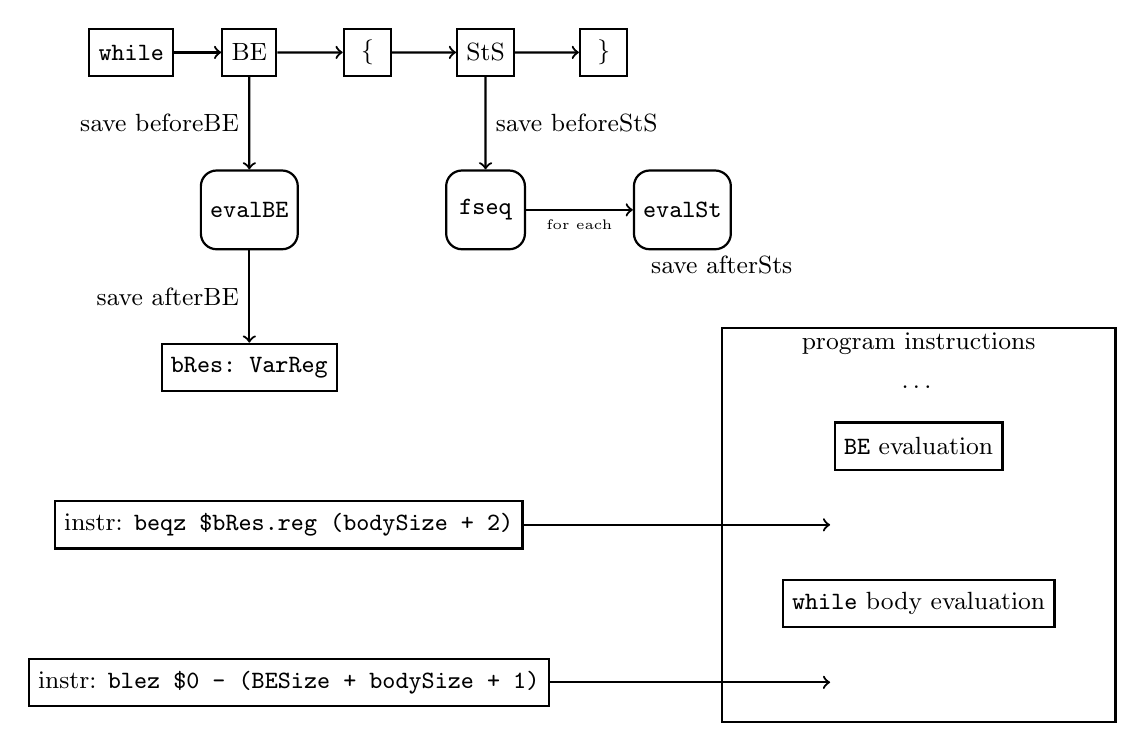
\begin{tikzpicture}
[font=\small,sibling distance =1.5cm, level distance=1.5cm, grow'=right, edge from parent/.style={draw=black, thick,->}]
\node[style A] (while) {\verb+while+}
child {
node[style A] (be) {BE}
child {
node[style A] (lcb) {\{}
child {
node[style A] (sts) {StS} child { node[style A] (rcb) {\}}}
}
}
};

\node[style B] at (1.5, -2) (evalBE) {\verb+evalBE+};
\node[style B] at (4.5, -2) (fseq) {\verb+fseq+};
\node[style B] at (7, -2) (evalSt) {\verb+evalSt+};
\node[draw=none] at (7.5, -2.7) (afterSts) {save afterSts};
\node[style A] at (1.5, -4) (bres) {\verb+bRes: VarReg+};
\node[style A] at (2, -6) (finstr) {instr: \verb_beqz $bRes.reg (bodySize + 2)_};
\node[style A] at (2, -8) (sinstr) {instr: \verb_blez $0 - (BESize + bodySize + 1)_};
\node[style A, minimum height=5cm, minimum width=5cm] at (10, -6) (box) {};
\node[draw=none] at (10,-3.7) (pinstr) {program instructions};
\node[draw=none] at (10, -4.25) (dots) {$\dots$};
\node[style A] at (10, -5) (beBody) {\verb_BE_ evaluation};
\node[draw=none] at (9, -6) (fjump) {};
\node[draw=none] at (9, -8) (sjump) {};
\node[style A] at (10, -7) (whileBody) {\verb_while_ body evaluation};

\draw[thick, ->] (be) -- node[midway,left] {\small save beforeBE} (evalBE);
\draw[thick, ->] (sts) -- node[midway, right] {\small save beforeStS} (fseq);
\draw[thick, ->] (fseq) -- node[midway, below] {\tiny for each} (evalSt);
\draw[thick, ->] (evalBE) -- node[midway, left] {\small save afterBE} (bres);
\draw[thick, ->] (finstr) -- (fjump);
\draw[thick, ->] (sinstr) -- (sjump);
\end{tikzpicture}
\caption{Evaluating loops}
\label{fig:while_st}
\end{figure}

\newpage
\subsection{If Statements}
Evaluation of the \verb+if+ statements has similarities with loops. Since there is a branch jump of the size
of the `if` body, the inner \verb+StS+ is evaluated first and the size of the body, index before the statement sequence
are recorded. Subsequently, branch instruction is inserted in the corresponding position in the list.
\begin{figure}[h]
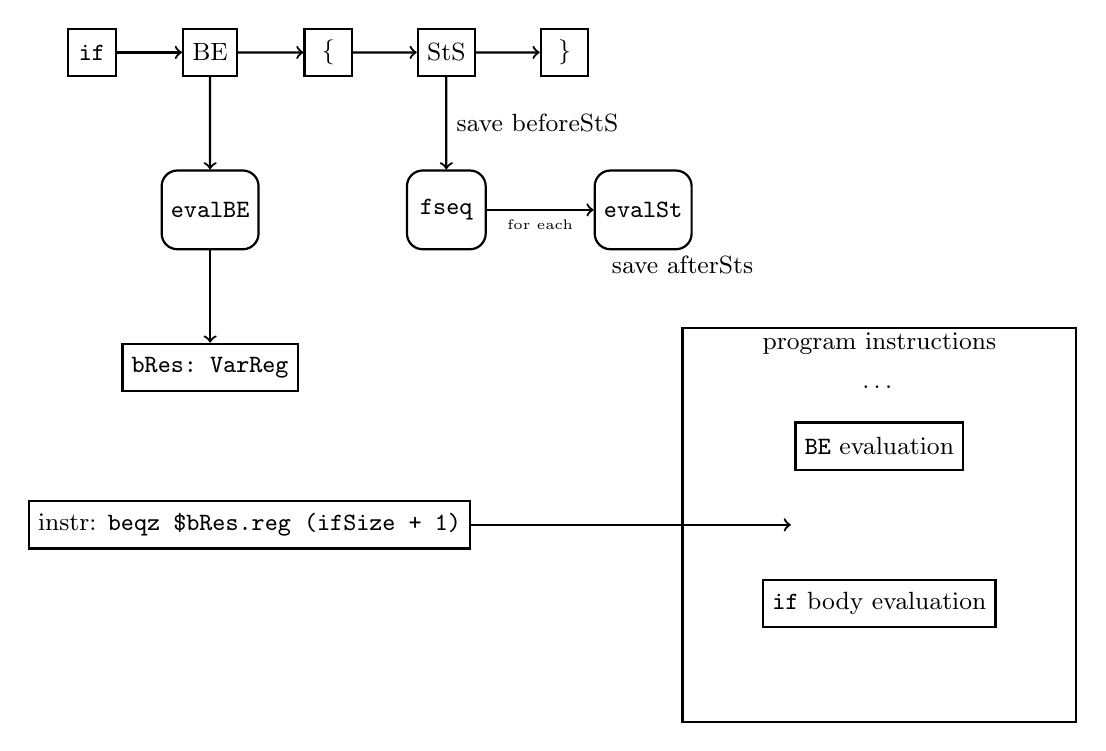
\begin{tikzpicture}
[font=\small,sibling distance =1.5cm, level distance=1.5cm, grow'=right, edge from parent/.style={draw=black, thick,->}]
\node[style A] (while) {\verb+if+}
child {
node[style A] (be) {BE}
child {
node[style A] (lcb) {\{}
child {
node[style A] (sts) {StS} child { node[style A] (rcb) {\}}}
}
}
};

\node[style B] at (1.5, -2) (evalBE) {\verb+evalBE+};
\node[style B] at (4.5, -2) (fseq) {\verb+fseq+};
\node[style B] at (7, -2) (evalSt) {\verb+evalSt+};
\node[draw=none] at (7.5, -2.7) (afterSts) {save afterSts};
\node[style A] at (1.5, -4) (bres) {\verb+bRes: VarReg+};
\node[style A] at (2, -6) (finstr) {instr: \verb_beqz $bRes.reg (ifSize + 1)_};
\node[style A, minimum height=5cm, minimum width=5cm] at (10, -6) (box) {};
\node[draw=none] at (10,-3.7) (pinstr) {program instructions};
\node[draw=none] at (10, -4.25) (dots) {$\dots$};
\node[style A] at (10, -5) (beBody) {\verb_BE_ evaluation};
\node[draw=none] at (9, -6) (fjump) {};
\node[draw=none] at (9, -8) (sjump) {};
\node[style A] at (10, -7) (whileBody) {\verb_if_ body evaluation};

\draw[thick, ->] (be) -- (evalBE);
\draw[thick, ->] (sts) -- node[midway, right] {\small save beforeStS} (fseq);
\draw[thick, ->] (fseq) -- node[midway, below] {\tiny for each} (evalSt);
\draw[thick, ->] (evalBE) -- (bres);
\draw[thick, ->] (finstr) -- (fjump);
\end{tikzpicture}
\caption{If statement evaluation}
\label{fig:if_st}
\end{figure}

\newpage
\subsection{If/Else Statements}
Only difference from the regular \verb+if+ statements is that an unconditional jump is added in the end of the
if body, to skip the else part. Given adjustments, initial branch jump's distance gets incremented. Other than that,
realization is straightforward.
\begin{center}
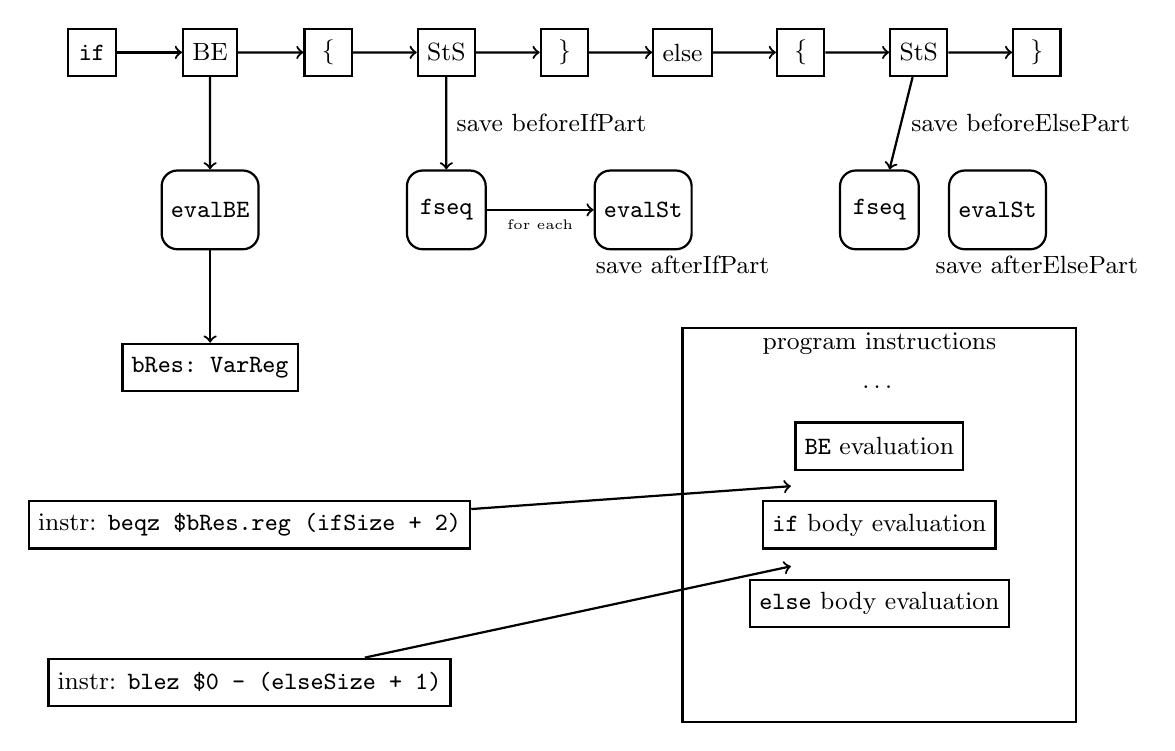
\begin{tikzpicture}
[font=\small,sibling distance =1.5cm, level distance=1.5cm, grow'=right, edge from parent/.style={draw=black, thick,->}]
\node[style A] (if) {\verb+if+}
child {
node[style A] (be) {BE}
child {
node[style A] (lcb) {\{} child {
node[style A] (ifsts) {StS} child {node[style A] (rcb) {\}} child {
node[style A] (else) {else} child {node[style A] (lcb1) {\{} child {
node[style A] (elsests) {StS} child {node[style A] (rcb1) {\}}}
}}
}}
}
}
};

\node[style B] at (1.5, -2) (evalBE) {\verb+evalBE+};
\node[style B] at (4.5, -2) (fseq) {\verb+fseq+};
\node[style B] at (7, -2) (evalSt) {\verb+evalSt+};
\node[draw=none] at (7.5, -2.7) (afterIfPart) {save afterIfPart};

\node[style B] at (10, -2) (fseq2) {\verb+fseq+};
\node[style B] at (11.5, -2) (evalSt2) {\verb+evalSt+};
\node[draw=none] at (12, -2.7) (afterElsePart) {save afterElsePart};


\node[style A] at (1.5, -4) (bres) {\verb+bRes: VarReg+};
\node[style A] at (2, -6) (finstr) {instr: \verb_beqz $bRes.reg (ifSize + 2)_};
\node[style A] at (2, -8) (sinstr) {instr: \verb_blez $0 - (elseSize + 1)_};
\node[style A, minimum height=5cm, minimum width=5cm] at (10, -6) (box) {};


\node[draw=none] at (10,-3.7) (pinstr) {program instructions};
\node[draw=none] at (10, -4.25) (dots) {$\dots$};
\node[style A] at (10, -5) (beBody) {\verb_BE_ evaluation};
\node[draw=none] at (9, -5.5) (fjump) {};
\node[draw=none] at (9, -6.5) (sjump) {};
\node[style A] at (10, -6) (ifBody) {\verb_if_ body evaluation};
\node[style A] at (10, -7) (elseBody) {\verb_else_ body evaluation};

\draw[thick, ->] (be) -- (evalBE);
\draw[thick, ->] (ifsts) -- node[midway, right] {\small save beforeIfPart} (fseq);
\draw[thick, ->] (elsests) -- node[midway, right] {\small save beforeElsePart} (fseq2);
\draw[thick, ->] (fseq) -- node[midway, below] {\tiny for each} (evalSt);
\draw[thick, ->] (evalBE) -- (bres);
\draw[thick, ->] (finstr) -- (fjump);
\draw[thick, ->] (sinstr) -- (sjump);
\end{tikzpicture}
\end{center}

\section{Translated programs}\label{sec:translated_programs}
In this section, we provide the translations of some programs written in C0 (Sample programs are copied from the system architecture book exercises on code generation \cite{sysbook}).
Listed programs are in c0 syntax, with the applied pre-processing (spaces and tabulations trimmed, dedicated `EOF` symbol appended),
whereas the compiled versions have jumps and links to the function label instead of the relative address, untranslated macros, the syscalls
used implicitly (e.g. HALT) and the comments for readability. With this in account, we delegate the complete translation of the program to the assembler.\\~\\
First example shows the program with assignments and conditional statements:
\begin{codeblock}
int x;
int main(){
x = 3;
x = x + 1;
if x>0 {x = 1} else {x = 2};
return 0
}~
\end{codeblock}
With it's respective translation:
\begin{codeblock}
_main:
addi $1 $28 0
addi $2 $2 3
sw $2 $1 0
addi $1 $28 0
addi $2 $28 0
lw $2 $2 0
addi $3 $3 1
add $2 $2 $3
sw $2 $1 0
addi $1 $28 0
lw $1 $1 0
addi $2 $2 0
sgt 1 1 2
beqz 1 4
addi $2 $28 0
addi $3 $3 1
sw $3 $2 0
addi $1 $1 0
HALT
\end{codeblock}

The program with a loop:
\begin{codeblock}
int n;
int res;
int main(){
n = 32768;
res = 0;
while n>0 {
res = res + n;
n = n - 1
};
return 0
}~
\end{codeblock}
Translated version:
\begin{codeblock}
_main:
addi $1 $28 0
addi $2 $2 32768
sw $2 $1 0
addi $1 $28 4
addi $2 $2 0
sw $2 $1 0
addi $1 $28 0
lw $1 $1 0
addi $2 $2 0
sgt 1 1 2
beqz 1 15
addi $2 $28 4
addi $3 $28 4
lw $3 $3 0
addi $4 $28 0
lw $4 $4 0
add $3 $3 $4
sw $3 $2 0
addi $1 $28 0
addi $2 $28 0
lw $2 $2 0
addi $3 $3 1
sub $2 $2 $3
sw $2 $1 0
blez 0 -18
addi $1 $1 0
HALT
\end{codeblock}
The program calculating the nth Fibonacci number:
\begin{codeblock}
int x;

int fib(int n){
int res;
int first;
int second;

if n<2 {res = n} else {
first = fib(n - 2);
second = fib(n - 1);
res = first + second
};

return res
};

int main(){
x=fib(31);
return 0
}~
\end{codeblock}
Translated version:
\begin{codeblock}
_main:
addi $1 $28 0
addi $2 $29 16 # start of increasing spt
subi $2 $2 32
blez 2 4
macro: gpr(1) = x
sysc
addi $29 $29 20 # end of increasing spt
add $2 $29 $-12
addi $3 $0 12
macro: zero($2, $3)
jal _fib
addi $1 $1 0
HALT

_fib:
addi $2 $0 -20
sw $31 $2 0
addi $2 $29 -16
lw $2 $2 0
addi $3 $3 2
slt $2 $2 $3
beqz 2 6
addi $3 $29 -12
addi $4 $29 -16
lw $4 $4 0
sw $4 $3 0
beq 0 30
addi $2 $29 -8
addi $3 $29 16 # start of increasing spt
subi $3 $3 32
blez 3 4
macro: gpr(1) = x
sysc
addi $29 $29 20 # end of increasing spt
add $3 $29 $-12
addi $4 $0 12
macro: zero($3, $4)
jal _fib
addi $3 $29 -4
addi $4 $29 16 # start of increasing spt
subi $4 $4 32
blez 4 4
macro: gpr(1) = x
sysc
addi $29 $29 20 # end of increasing spt
add $4 $29 $-12
addi $5 $0 12
macro: zero($4, $5)
jal _fib
addi $4 $29 -12
addi $5 $29 -8
lw $5 $5 0
addi $6 $29 -4
lw $6 $6 0
add $5 $5 $6
sw $5 $4 0
addi $4 $29 -12
lw $4 $4 0
sw $4 $1 0 # start of return from fib
lw $1 $29 -20
addi $29 $29 -20
jr 1 # end of return from fib
\end{codeblock}
\newpage
The program calculating powers, using the defined struct:
\begin{codeblock}
typedef struct {int exp; int val} powst;
int x;

int main(){
x=pow(2, 2);
return x
};

int pow(int base, int n){
powst p;
p = new powst*;
p.exp = 0;
p.val = 1;
while p.exp<n {
p.exp = p.exp + 1;
p.val = p.val*base
};
return p.val
}~
\end{codeblock}
Translation:
\begin{codeblock}
_main:
addi $1 $28 0
addi $2 $29 16 # start of increasing spt
subi $2 $2 32
blez 2 4
macro: gpr(1) = x
sysc
addi $29 $29 20 # end of increasing spt
addi $2 $2 2
sw $2 $29 -16
addi $2 $2 2
sw $2 $29 -12
add $2 $29 $-8
addi $3 $0 8
macro: zero($2, $3)
jal _pow
addi $1 $28 0
lw $1 $1 0
HALT

_pow:
addi $2 $0 -20
sw $31 $2 0
addi $2 $29 -8
sw $30 $2 0
# INCREASING HEAP POINTER
addi $30 $30 8 # start of increasing hpt
subi $1 $30 31
bltz 1 4
macro: gpr(1) = x
sysc
addi $1 $30 -8
addi $2 $0 2
zero(1, 2) # end of increasing hpt
addi $2 $29 -8
addi $2 $2 0
addi $3 $3 0
sw $3 $2 0
addi $2 $29 -8
addi $2 $2 4
addi $3 $3 1
sw $3 $2 0
addi $2 $29 -8
addi $2 $2 0
lw $2 $2 0
addi $3 $29 -12
lw $3 $3 0
slt $2 $2 $3
beqz 2 19
addi $3 $29 -8
addi $3 $3 0
addi $4 $29 -8
addi $4 $4 0
lw $4 $4 0
addi $5 $5 1
add $4 $4 $5
sw $4 $3 0
addi $2 $29 -8
addi $2 $2 4
addi $3 $29 -8
addi $3 $3 4
lw $3 $3 0
addi $4 $29 -16
lw $4 $4 0
macro: mul($3, $3, $4)
sw $3 $2 0
blez 0 -24
addi $2 $29 -8
addi $2 $2 4
lw $2 $2 0
sw $2 $1 0 # start of return from pow
lw $1 $29 -20
addi $29 $29 -20
jr 1 # end of return from pow
\end{codeblock}
\newpage
Linked lists:
\begin{codeblock}
typedef LEL* u;
typedef struct {int content; u next} LEL;
u first;
u last;
int n;
int main(){
n = 200;
first = new LEL*;
last = first;
n = n -1;
while n>0 {
last*.next = new LEL*;
last = last*.next;
n = n - 1
};
return 0
}~
\end{codeblock}
Translation:
\begin{codeblock}
_main:
addi $1 $28 8
addi $2 $2 200
sw $2 $1 0
addi $1 $28 0
sw $30 $1 0
# INCREASING HEAP POINTER
addi $30 $30 4 # start of increasing hpt
subi $1 $30 31
bltz 1 4
macro: gpr(1) = x
sysc
addi $1 $30 -4
addi $2 $0 1
zero(1, 2) # end of increasing hpt
addi $1 $28 4
addi $2 $28 0
lw $2 $2 0
sw $2 $1 0
addi $1 $28 8
addi $2 $28 8
lw $2 $2 0
addi $3 $3 1
sub $2 $2 $3
sw $2 $1 0
addi $1 $28 8
lw $1 $1 0
addi $2 $2 0
sgt 1 1 2
beqz 1 27
addi $2 $28 4
lw $2 $2 0
addi $2 $2 4
sw $30 $2 0
# INCREASING HEAP POINTER
addi $30 $30 4 # start of increasing hpt
subi $1 $30 31
bltz 1 4
macro: gpr(1) = x
sysc
addi $1 $30 -4
addi $2 $0 1
zero(1, 2) # end of increasing hpt
addi $1 $28 4
addi $2 $28 4
lw $2 $2 0
addi $2 $2 4
lw $2 $2 0
sw $2 $1 0
addi $1 $28 8
addi $2 $28 8
lw $2 $2 0
addi $3 $3 1
sub $2 $2 $3
sw $2 $1 0
blez 0 -30
addi $1 $1 0
HALT
\end{codeblock}

    \begin{thebibliography}{9}
        \bibitem{sysbook}
        Wolfgang J. Paul, Christoph Baumann, Petro Lutsyk, Sabine Schmaltz (2016) System Architecture: An Ordinary Engineering Discipline

        \bibitem{sipser}
        Michael Sipser (2013) Introduction to the Theory of Computation

        \bibitem{DFA}
        "NFA and DFA Equivalence Theorem Proof, Conversion Algorithm and Example"
        by Neural Dump. \href{https://neuraldump.net/2017/11/nfa-and-dfa-equivalence-theorem-proof-and-example/}{Link}
    \end{thebibliography}
\end{document}